\documentclass{tktltiki}
\usepackage{url}
\begin{document}
\title{Keskitetty tunnistautuminen web-sovelluksissa}
\author{Olli Jokinen}
\date{\today}
\level{Pro gradu -tutkielma}
\maketitle
\doublespacing
\faculty{Matemaattis-luonnontieteellinen}
\department{Tietojenkäsittelytieteen laitos}
\subject{Tietojenkäsittelytiede}
\depositeplace{Tietojenkäsittelytieteen laitoksen kirjasto}
\additionalinformation{}
\numberofpagesinformation{\numberofpages\ sivua +
\numberofappendixpages[100] liitesivua}
\classification{A.1 [Introductory and Survey] \\
I.7.m [Document and Text Processing]: Miscellaneous}
\keywords{avainsana}
\begin{abstract}
Tutkielmassa selvitetään keskitetyn tunnistautumispalvelun toteuttamista palvelusuuntautuneiden arkkitehtuurien mukaisissa web-sovellusympäristöissä. Pääpainopisteenä on sovellusympäristöt, joissa ollaan siirtymässä palvelusuuntautuneisiin arkkitehtuureihin. Tutkielmassa käytetään esimerkkinä tällaisesta ympäristöstä Kapsi Internet-käyttäjät ry:n jäsenhallintatyökaluja, joiden tunnistautuminen muutetaan keskitetyn tunnistautumispalvelun tehtäväksi.

Web-sovellusten kehitys ensimmäisistä CGI-ohjelmista kohti palvelusuuntautuneita arkkitehtuureita ja tunnistautumisen tarpeet tällaisissa arkkitehtuureissa esitellään. Tutkielmassa käydään läpi turvallisuuden osatekijöitä ja tavallisia tunnistautumiseen liittyviä ongelmia web-sovelluksissa. Hahmotellaan keskitetty tunnistautumispalvelu ratkaisemaan ongelmia sekä pohditaan sen etuja ja haittoja nykyään käytettyihin tunnistautumismekanismeihin nähden.

Tunnistautumispalvelun ja web-sovelluksen väliseen rajapintaan käytettäviä protokollia (SAML, OpenID ja OAuth) tutkitaan ja esitellään OAuth-protokollaa käyttävä arkkitehtuuri Kapsin järjestelmään. Esitetyn arkkitehtuurin etuja ja haittoja sekä sen soveltamista muihin vastaaviin ympäristöihin tutkitaan. Arkkitehtuurin laajentamista keskitettyyn pääsynvalvontaan ja kertakirjautumiseen pohditaan. Ulkoisen tunnistautumispalvelun käyttöä pohditaan, esimerkkinä Facebookin tarjoama tunnistautumisrajapinta.
\end{abstract}
\mytableofcontents
\section{Johdanto}
Miten käyttäjädataa onko käsitelty ja käsitellään. Kehitys paikallisesti käytetyistä tiedostopohjaisista systeemeistä kohti tietokantoja ja asiaan räätälöihin palveluihin (LDAP). LDAP oleelisin, mutta tutkimuksen kannalta abstraktointi on tärkeä juttu.

Johdanto puoli sivua, alaluvut 0.5-1 sivu.
\section{Web-sovellukset}
Miten käyttäjädataa onko käsitelty ja käsitellään. Kehitys paikallisesti käytetyistä tiedostopohjaisista systeemeistä kohti tietokantoja ja asiaan räätälöihin palveluihin (LDAP). LDAP oleelisin, mutta tutkimuksen kannalta abstraktointi on tärkeä juttu.

Johdanto puoli sivua, alaluvut 0.5-1 sivu.
\subsection{Historia}
WWW:n, ja erityisesti WWW:n edeltäjän Gopherin, sivustot olivat alkujaan lähinnä staattisia dokumentteja, jotka oli linkitetty toisiinsa. Dokumentit muodostivat erillisia arkistoja esimerkiksi tutkijoiden käyttöön. Ajan kuluessa tuli tarpeelliseksi tehdä sivustoja, jotka reagoivat käyttäjän syötteeseen ja toimivat dynaamisesti käyttäjän syötteen mukaan.

Vuonna 1993 esitelty Common Gateway Interface (CGI) on standardi, jolla voidaan ajaa ohjelmia web-sivujen kautta UNIX-ympäristössä \cite{rfc3875}. Tyypillisesti CGI:llä ajettavat ohjelmat ovat itsenäisiä ja ne on kirjoitettu jollain skriptikielellä esimerkiksi Perlillä tai PHP:lla. Skripti saa parametrina käyttäjän lähettämät syötteet ja muodostaa sen perusteella käyttäjälle näkyvän HTML-sivun. Ajan kuluessa CGI-ohjelmat alkoivat kasvaa ja niiden arkkitehtuuri monimutkaistua, kun esimerkiksi niissä alettiin käyttää tietokantoja.

CGI-ohjelmien kasvun lisäksi myös niiden suoritukseen vaadittava ajoympäristö alkoi kasvaa ja muodostaa ongelmia CGI:n käytölle. CGI käynnistää suoritettavan prosessin jokaisen sivupyynnön yhteydessä, mikä voi olla hidasta, jos prosessi esimerkiksi lataa muistiin paljon dataa. Erityisesti 1990-luvulla Sunin kehittämä Java-kieli, joka saavutti suosiota web-kehittäjien keskuudessa, oli merkittävässä roolissa 1990-luvun lopun web-kehityksessä \cite{uml}.

Javan web-käyttöön suunniteltu Enterprise Edition (J2EE) käyttää Servlet-tekniikkaa, joka laajentaa perinteisen web-palvelimen toimintaa. Servlet-ohjelmia ei siis käynnistetä erillisestä web-palvelimesta, vaan se suoritetaan web-palvelimen sisällä. Käyttäjän pyynnön saatuaan web-palvelin (esimerkiksi Apache Tomcat) ohjaa pyynnön Java Servetille, joka käsiteltyään sen, palauttaa vastauksen web-palvelimelle, joka näyttää sivun käyttäjälle. Web-palvelin pitää siis Java-prosessia kokoajan käynnissä ja ympäristöä ei tarvitse käynnistää jokaisen käyttäjän pyynnön yhteydessä uudestaan. Servlet-tekniikan avulla voidaan tehostaa resurssien jakamista useamman pyynnön kesken, tehdä transaktioimalleja, muuttaa käyttäjäohjelman tilaa ja hallita web-sovelluksia etänä \cite{uml}. Eri kielille on toteutettu myös omia, Javan Servlettiä muistuttavia, web-palvelimia, esimerkiksi Ruby on Rails web-ohjelmointikehys tarjoaa oletuksena Rubyyn sisäänrakennetun WEBrick web-palvelimen, joka käynnistää ympäristön ja ohjaa pyynnöt oikeille Ruby on Rails -luokille \cite{ruby2011agile}. Kuvassa \ref{servlet} on kuvattu yksittäisen sivupyynnön kulkua Java Servlet-palvelimessa.

\begin{figure}[ht]
\centering
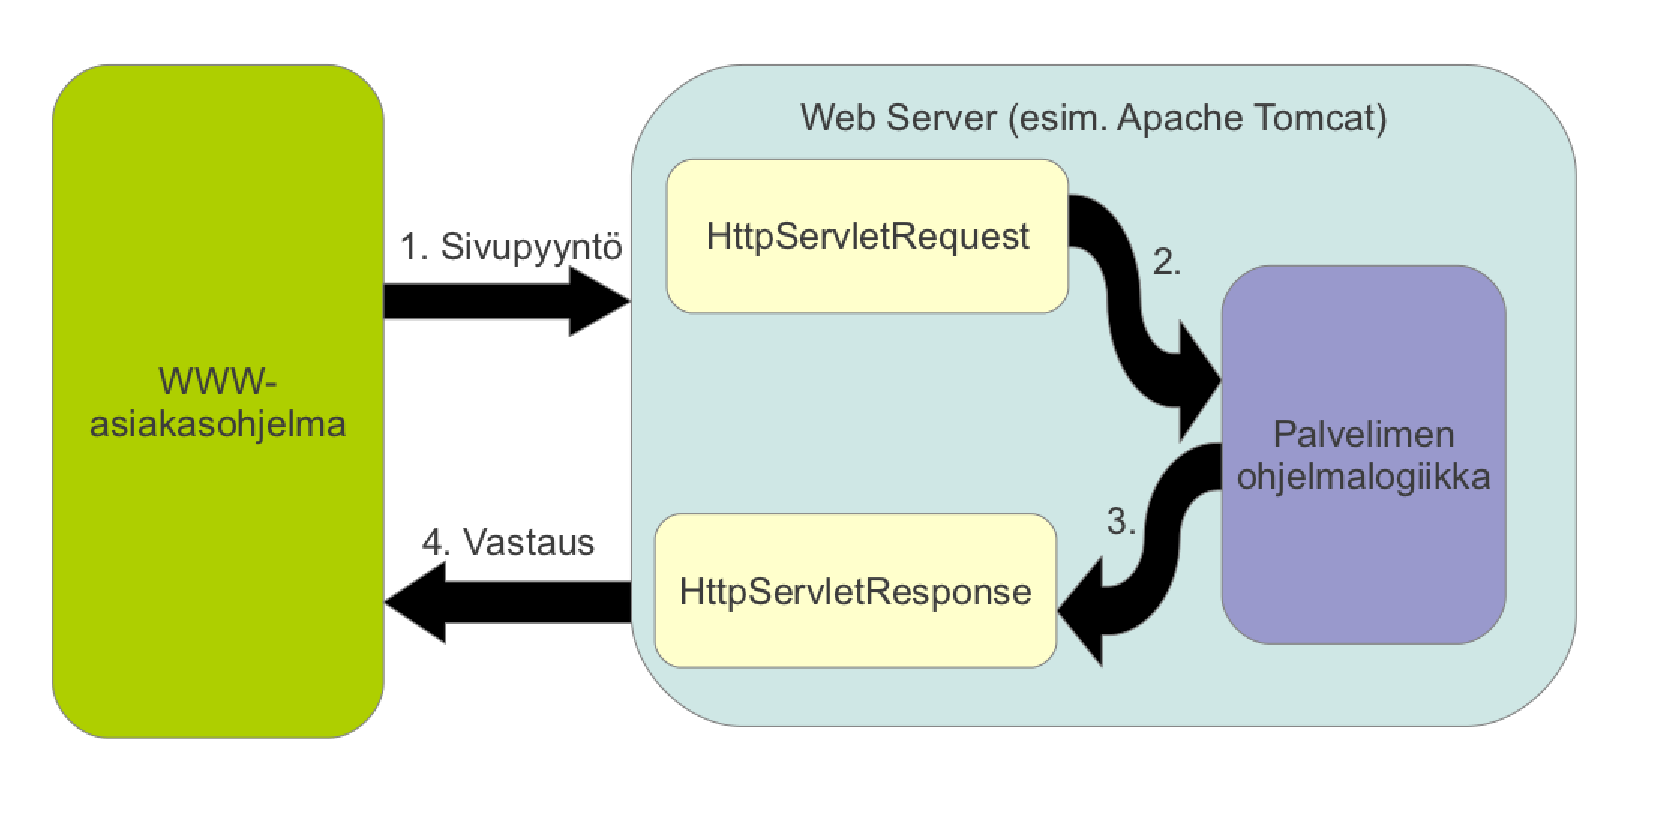
\includegraphics[width=\textwidth]{web/servlet.eps}
\caption{Kontrollin kulku Java Servlet-palvelimessa}%
\label{servlet}
\end{figure}

Servletien jälkeen paljon suosiota on saanut CGI:stä kehittynyt FastCGI-protokolla, joka korjaa CGI:ssä havaittuja puutteita \cite{fastcgi}. Web-palvelin ei käynnistä jokaista pyyntöä kohti uutta prosessia, vaan pyynnöt lähetetään ja vastaanotetaan pistokkeen (socket) avulla palvelimella suoritettavalle prosessille. FastCGI-ohjelmat voivat olla myös hajautettu eri palvelimille, jolloin pyyntöjen välitykseen käytetään TCP-yhteyttä. FastCGI:tä voidaan käyttää minkä tahansa kielen kanssa, joka tukee pistokkeiden käyttöä. Näin ollen se on varteenotettava tekniikka, koska ohjelmointikieli ei ole rajattu vain Javaan, vaan käytössä on Javan lisäksi koko kielien kirjo (esimerkiksi PHP, Python ja Ruby).

Tiivistetysti web-sovellusten historiasta voidaan sanoa, että niistä on tullut itsenäisiä ohjelmia, jotka pyörivät jatkuvasti palvelimella. Ohjelmat saavat kontrollin web-palvelimelta, joko laajentamalla web-palvelimen toimintaa (Servlet, WEBrick yms) tai pistokkeiden avulla (FastCGI). Web-sovellukset tuottavat käyttäjän syötteen ja web-sovelluksen sen hetkisen tilan mukaan käyttäjälle dynaamisen HTML tms muotoisen sivun. Seuraavissa kappaleissa pureudutaan web-sovellusten arkkitehtuuriin ja tutkitaan niiden kehitystä.
\subsection{Web-sovellusten arkkitehtuuri}
Servlet- tai FastCGI-tekniikka ei sido web-sovelluksen arkkitehtuuria, vaan molempia tekniikoita käytettäessä sovellusten perusarkkitehtuuri on sama. Sovellukset ovat jatkuvasti pyöriviä prosesseja, jotka saavat syötteenään käyttäjän syöttämän datan lisäksi joukon erilaisia suoritusympäristöön liittyviä resursseja ja muuttujia (mm. tietokantayhteys) \cite{uml}. Syötteen perusteella sovellus tuottaa tulosteen, joka palautetaan käyttäjälle.

Tyypillinen tapa toteuttaa web-sovelluksia nykypäivänä on käyttää sovelluskehystä, joka tuo oman lisänsä sovellusten arkkitehtuuriin. Käytettyjä kehyksiä on esimerkiksi Javalla toteutettu Spring, Pythonin Django ja Ruby-ohjelmointikieleen luottava Ruby on Rails. Näissä sovelluskehyksissä erillinen viestinvälittäjä (dispatcher) ottaa vastaan pyynnön ja välittää sen eteenpäin sovellusohjelmalle. Pyyntö ei siirry suoraan sovellusohjelmalle, vaan se välitetään väliohjelma-kerroksen läpi \cite{ruby2011agile}. Nämä väliohjelmat esimerkiksi tekevät merkintöjä lokitiedostoihin, asettavat ja lukevat käyttäjän selaimen evästeitä tai asettavat ympäristömuuttujia sovellusohjelmaa varten.

TODO: kuva vaikka railsin dispatcherista

Sovellusohjelmasta on pyritty karsimaan paljon yleisiä tehtäviä sovelluskehyksen tai käyttäjän toteuttaman väliohjelman tehtäväksi. Web-sovellusohjelman toteuttaja käyttää hyväkseen sovelluskehyksen tarjoamia ympäristömuuttujia, jotka ovat esimerkiksi viittauksia muuttujiin, joita säilytetään istunnon (session) ajan muistissa. Myös käyttäjän tunnistautuminen on yksi sovelluskehyksen tehtävistä, sovellusohjelma saa ympäristömuuttujana kirjautuneen käyttäjän tiedot (esimerkiksi tunnistenumeron ja käyttöoikeudet), joita se käyttää hyväksi ohjelmalogiikassaan.

Sovelluskehysten otettua vastuun web-sovellusten perustoiminallisuudesta on web-sovellusten arkkitehtuuri mennyt modulaarisempaan suuntaan [TODO: lähde?]. Saman sovelluskehyksen sisällä voi olla useampia ohjelmamoduuleita, joita viestinvälittäjä kutsuu esimerkiksi URL-osoitteen perusteella. Kun ohjelmamoduuleiden ei tarvitse toteuttaa kaikkea perustoiminallisuutta itse, yksinkertaistuu niiden rakenne ja web-sovellusten arkkitehtuureissa voidaan mennä kohti palveluperustaisia arkkitehtuureja.
\subsection{Palveluperustaiset arkkitehtuurit}
Perus arkkitehtuurissa oleva sovellus pilkotaan autonomisiin kokonaisuuksiin, jotka juttelee keskenään web service -rajapintojen kautta.

tässä kai voisi kertoa kehityksen perus server-client moskasta kohti javascriptillä toteutettavia DOM-virityksiä

Erityisesti tärkeää kertoa, että käyttöliittymä ja data erotetaan toisistaan: käyttöliittymä rakennetaan javascriptillä (tai flashilla, silverlightilla whatever) ja erilliset palvelut tarjoavat sitten json/xml-dataa, jota tuo käyttöliittymä visualisoi. Gradun ongelma onkin juuri tässä: miten toteuttaa käyttöliittymä, jossa javascript hakee dataa erilaisista datalähteistä ja käyttäjä pystytään tunnistamaan näissä eri datalähteissä. Tuskin tämä kuuluu web-palveluiden historia-kappaleeseen, mutta tämän kappaleen tarkoitus on kertoa lukijalle, että tällaisia ne web-palvelut nykyään on. Eli n-tier on tässä nyt jotenkin läsnä.
\subsection{Yhteenveto}
Keskitetyn tunnistautumispalvelun käyttö on perusteltua, jos ympäristössä on useita käyttäjän tunnistamista vaativia web-sovelluksia. Tunnistautumispalvelun käytöllä ehkäistään käyttäjätietojen kopiointiin liittyviä synkronointiongelmia, kun käyttäjädata on keskitetty yhteen paikkaan. Erityisesti arkaluontoinen data, kuten salasanatiivisteet, kannattaa keskittää, jolloin ne eivät päädy vääriin käsiin yksittäisiin web-sovelluksiin kohdistuneiden tietomurtojen yhteydessä.

Tunnistautumispalvelu mahdollistaa myös muiden kuin järjestelmän ylläpitäjien tuottamien sovellusten käytön organisaation sisäisillä käyttäjätunnuksilla. Käyttämällä luotettavaksi todettuja rajapintoja, voi ylläpito antaa kolmannen osapuolen toteuttamalle web-sovellukselle oikeuden käyttää tunnistautumispalvelua käyttäjän tunnistamiseen. Tällöin käyttäjä ohjataan tunnistautumispalveluun tunnistamisen ajaksi ja web-sovellus saa vain pääsyvaltuuden, jolla sovellus voi hakea käyttäjän tiedot. Käyttäjän tunnistetiedot eivät tule missään vaiheessa tunnistamista tarvitsevan web-sovelluksen tietoon. Näin ollen esimerkiksi Facebook-tunnuksilla voi kirjautua useaan web-sovellukseen, vaikka Facebookilla ei ole tarkkaa tietoa sovelluksien sisäisestä toimintalogiikasta.

Tutkielmassa esitellyn Kapsi ry:n hallintatyökalujen tapauksessa palvelu tullaan toteuttamaan Django-sovelluskehyksellä, mutta myös valmiita toteutuksia on olemassa eri intranet-ympäristöihin. Teknologivalinta tulee tehdä sovellusympäristön mukaan, eikä yksi ratkaisu sovi kaikkiin ympäristöihin. Web-sovelluksen ja tunnistautumispalvelun välinen rajapinta pitää huolen palveluiden yhteensopivuudesta. Rajapinnoiksi on valittavissa useita eri protokollia, kuten Web Services -standardin SAML tai avoimen lähdekoodin yhteisössä syntyneet OpenID ja OAuth. Protokollien käyttö rinnakkain on myös mahdollista, jolloin tunnistautuminen voidaan tehdä esimerkiksi SAML- tai OAuth-protokollalla riippuen web-sovelluksesta.

Tunnistautumiseen liittyvien tehtävien erottaminen yksittäisiltä web-sovelluksilta erillisen palvelun tehtäväksi on palvelusuuntauneiden arkkitehtuurien periaatteiden mukaista. Tällaisten arkkitehtuurien mukaan toteutetuissa sovellusympäristöissä jokaisella web-sovelluksella on oma tarkasti määritelty tehtävä. Kun arkkitehtuurissa on oma palvelu tunnistautumiselle, on pienten yksittäisten komponenttien toteutus helpompaa, koska jokaisen komponentin kohdalla ei tarvitse huolehtia tunnistautumisen toteutuksesta.

Web-sovelluksen ja tunnistamisen erottaminen toisistaan mahdollistaa myös tunnistautumisen tehostamisen ilman muutoksia web-sovellusten toimintaan. Järjestelmässä voidaan ottaa salasanan lisäksi käyttöön toiseen tekijään perustuva tunnistaminen, jolloin esimerkiksi käyttäjän täytyy salasanan lisäksi syöttää matkapuhelimeen lähetetty tunnistekoodi. Web-sovelluksen ja tunnistautumispalvelun välinen rajapinta ei tässä tapauksessa muutu, joten tunnistamisen parantaminen ei edellytä web-sovelluksien muuttamista.

Keskitetyn pääsynvalvonnan toteuttaminen tutkielmassa kuvatuilla periaatteilla on mahdollista. Tällöin tiedot käyttäjien pääsyoikeuksista ympäristön sisällä ovat yhdessä paikassa, joka helpottaa niiden hallinnointia. Esimerkiksi henkilön siirtyessä tehtävästä toiseen, voidaan hänen pääsyvaltuudet muuttaa samasta paikasta. Pääsynvalvontaan voidaan käyttää esimerkiksi tutkielmassa esiteltyjä SAML- tai OAuth-protokollia.

Käyttäjän tunnistamista vaativissa web-sovelluksissa käyttäjän tunnistaminen kannattaa toteuttaa erillisenä komponenttina. Käytettyjen teknologioiden suhteen valinta täytyy tehdä web-sovellusympäristön mukaan, koska kaikkiin ympäristöihin sopivaa ratkaisua ei ole. Tässä tutkielmassa esitellyt periaatteet ovat kuitenkin sovellettavissa eri teknologioita käytettäessä.

\section{Tunnistautuminen}
Miten käyttäjädataa onko käsitelty ja käsitellään. Kehitys paikallisesti käytetyistä tiedostopohjaisista systeemeistä kohti tietokantoja ja asiaan räätälöihin palveluihin (LDAP). LDAP oleelisin, mutta tutkimuksen kannalta abstraktointi on tärkeä juttu.

Johdanto puoli sivua, alaluvut 0.5-1 sivu.
\subsection{Termistö}
Miten käyttäjädataa onko käsitelty ja käsitellään. Kehitys paikallisesti käytetyistä tiedostopohjaisista systeemeistä kohti tietokantoja ja asiaan räätälöihin palveluihin (LDAP). LDAP oleelisin, mutta tutkimuksen kannalta abstraktointi on tärkeä juttu.

Johdanto puoli sivua, alaluvut 0.5-1 sivu.
\subsubsection{Asiakas}
Palvelun käyttäjä, joka tunnistautuu palveluun. Tyypillisesti HTTP-asiakas, joka tunnistautuu palveluun selaimen avustuksella.
\subsubsection{Tunnistautumispalvelin}
HTTP-palvelu, johon käyttäjä ohjataan tekemään tunnistautuminen. Onnistuneen tunnistautumisen jälkeen palvelin ohjaa takaisin tunnistautumista pyytäneen palvelun määrittelemään osoitteeseen. Avoimen Internetin puolella tunnistautumispalvelu voi olla esimerkiksi Facebook tai LinkedIn.
\subsubsection{Suojattu resurssi}
Tunnistautumisprotokollien yhteydessä suojatulla resurssilla tarkoitetaan resurssia, jonka käyttö vaatii tunnistautumisen ja käyttöoikeuden. Tämän tutkielman puitteissa suojatulla resurssilla tarkoitetaan tunnistautumista vaativaa web-palvelua. Tutkielman laajennusosassa (luku 7) kuvataan esitetyn prototyypin laajentamista myös yksittäisten resurssien (käyttäjän valokuva tms) pääsynvalvontaan.
\subsubsection{Valtuutustieto (crendentials)}
Valtuutustieto (credentials) koostuu yksilöivästä tunnisteesta ja siihen liittyvästä salaisesta avaimesta. Tämän tutkielman puitteissa valtuutustiedolla tarkoitetaan käyttäjän tunnusta ja salasanaa.
\subsubsection{Valtuutusavain (token)}
Pääsyvaltuutus (access token) on tunnistautumispalvelimelta saatava yksilöivä tunniste, jonka avulla suojatun resurssin omistaja voi pyytää käyttäjän tiedot tunnistautumispalvelulta. Pääsyvaltuutus on voimassa tietyn ajan, jonka jälkeen se täytyy uusia tunnistautumispalvelimella. Tutkielmassa toteutettavassa prototyypissä tunnistautumispalvelu sisältää myös käyttäjän hallinnan, mutta yleisessä tapauksessa pääsyvaltuutusta voidaan käyttää myös tunnistautumispalvelusta erillään olevien resurssien valtuuttamiseen.
\subsection{Tunnistautumisen historia}
WWW:n, ja erityisesti WWW:n edeltäjän Gopherin, sivustot olivat alkujaan lähinnä staattisia dokumentteja, jotka oli linkitetty toisiinsa. Dokumentit muodostivat erillisia arkistoja esimerkiksi tutkijoiden käyttöön. Ajan kuluessa tuli tarpeelliseksi tehdä sivustoja, jotka reagoivat käyttäjän syötteeseen ja toimivat dynaamisesti käyttäjän syötteen mukaan.

Vuonna 1993 esitelty Common Gateway Interface (CGI) on standardi, jolla voidaan ajaa ohjelmia web-sivujen kautta UNIX-ympäristössä \cite{rfc3875}. Tyypillisesti CGI:llä ajettavat ohjelmat ovat itsenäisiä ja ne on kirjoitettu jollain skriptikielellä esimerkiksi Perlillä tai PHP:lla. Skripti saa parametrina käyttäjän lähettämät syötteet ja muodostaa sen perusteella käyttäjälle näkyvän HTML-sivun. Ajan kuluessa CGI-ohjelmat alkoivat kasvaa ja niiden arkkitehtuuri monimutkaistua, kun esimerkiksi niissä alettiin käyttää tietokantoja.

CGI-ohjelmien kasvun lisäksi myös niiden suoritukseen vaadittava ajoympäristö alkoi kasvaa ja muodostaa ongelmia CGI:n käytölle. CGI käynnistää suoritettavan prosessin jokaisen sivupyynnön yhteydessä, mikä voi olla hidasta, jos prosessi esimerkiksi lataa muistiin paljon dataa. Erityisesti 1990-luvulla Sunin kehittämä Java-kieli, joka saavutti suosiota web-kehittäjien keskuudessa, oli merkittävässä roolissa 1990-luvun lopun web-kehityksessä \cite{uml}.

Javan web-käyttöön suunniteltu Enterprise Edition (J2EE) käyttää Servlet-tekniikkaa, joka laajentaa perinteisen web-palvelimen toimintaa. Servlet-ohjelmia ei siis käynnistetä erillisestä web-palvelimesta, vaan se suoritetaan web-palvelimen sisällä. Käyttäjän pyynnön saatuaan web-palvelin (esimerkiksi Apache Tomcat) ohjaa pyynnön Java Servetille, joka käsiteltyään sen, palauttaa vastauksen web-palvelimelle, joka näyttää sivun käyttäjälle. Web-palvelin pitää siis Java-prosessia kokoajan käynnissä ja ympäristöä ei tarvitse käynnistää jokaisen käyttäjän pyynnön yhteydessä uudestaan. Servlet-tekniikan avulla voidaan tehostaa resurssien jakamista useamman pyynnön kesken, tehdä transaktioimalleja, muuttaa käyttäjäohjelman tilaa ja hallita web-sovelluksia etänä \cite{uml}. Eri kielille on toteutettu myös omia, Javan Servlettiä muistuttavia, web-palvelimia, esimerkiksi Ruby on Rails web-ohjelmointikehys tarjoaa oletuksena Rubyyn sisäänrakennetun WEBrick web-palvelimen, joka käynnistää ympäristön ja ohjaa pyynnöt oikeille Ruby on Rails -luokille \cite{ruby2011agile}. Kuvassa \ref{servlet} on kuvattu yksittäisen sivupyynnön kulkua Java Servlet-palvelimessa.

\begin{figure}[ht]
\centering
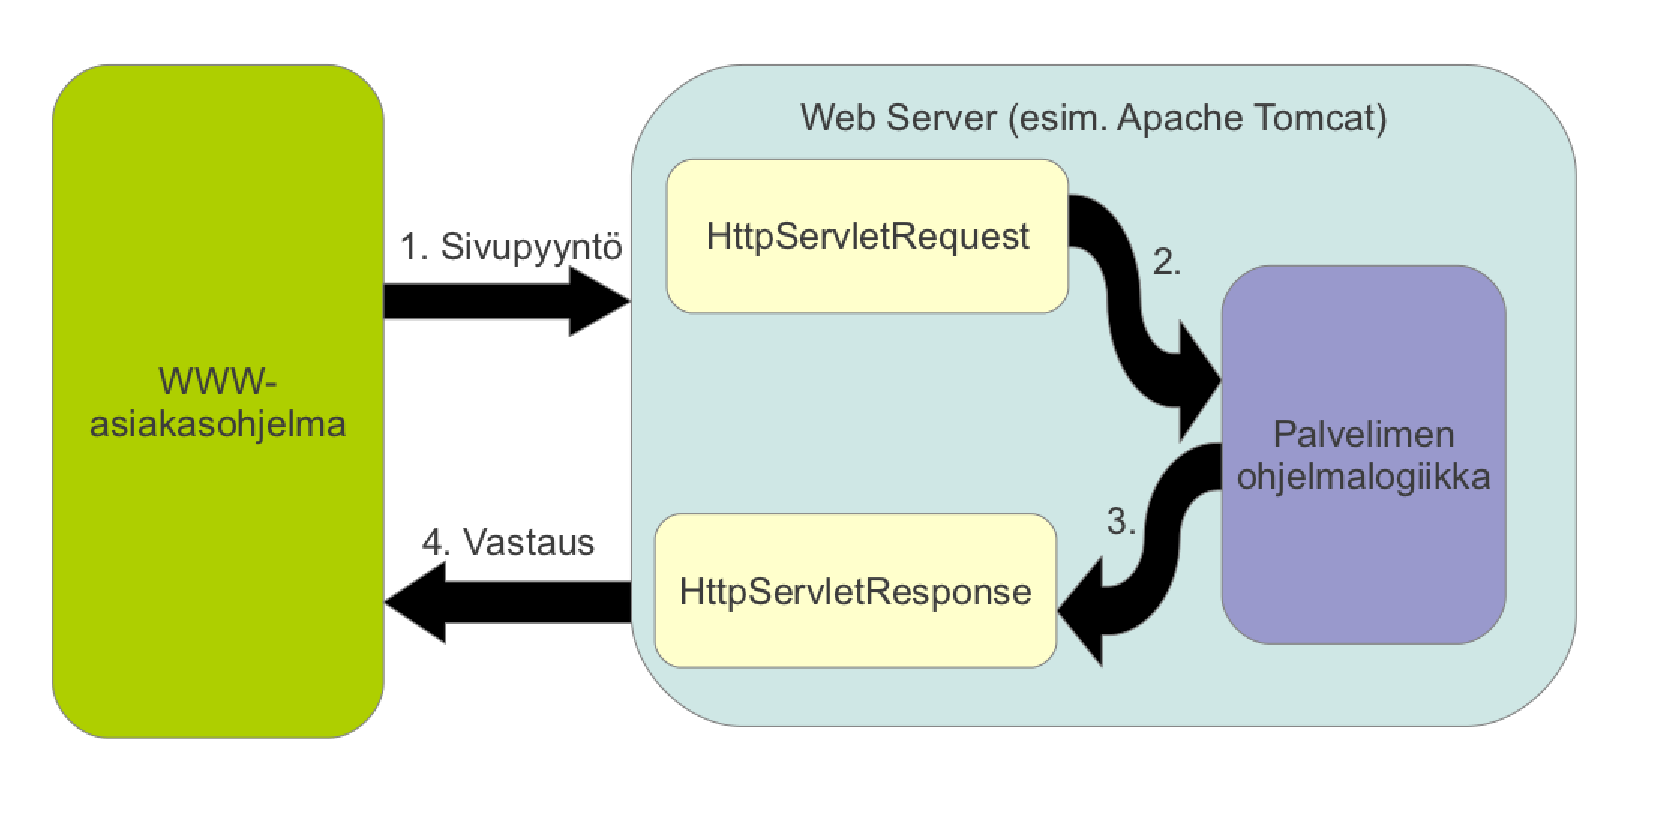
\includegraphics[width=\textwidth]{web/servlet.eps}
\caption{Kontrollin kulku Java Servlet-palvelimessa}%
\label{servlet}
\end{figure}

Servletien jälkeen paljon suosiota on saanut CGI:stä kehittynyt FastCGI-protokolla, joka korjaa CGI:ssä havaittuja puutteita \cite{fastcgi}. Web-palvelin ei käynnistä jokaista pyyntöä kohti uutta prosessia, vaan pyynnöt lähetetään ja vastaanotetaan pistokkeen (socket) avulla palvelimella suoritettavalle prosessille. FastCGI-ohjelmat voivat olla myös hajautettu eri palvelimille, jolloin pyyntöjen välitykseen käytetään TCP-yhteyttä. FastCGI:tä voidaan käyttää minkä tahansa kielen kanssa, joka tukee pistokkeiden käyttöä. Näin ollen se on varteenotettava tekniikka, koska ohjelmointikieli ei ole rajattu vain Javaan, vaan käytössä on Javan lisäksi koko kielien kirjo (esimerkiksi PHP, Python ja Ruby).

Tiivistetysti web-sovellusten historiasta voidaan sanoa, että niistä on tullut itsenäisiä ohjelmia, jotka pyörivät jatkuvasti palvelimella. Ohjelmat saavat kontrollin web-palvelimelta, joko laajentamalla web-palvelimen toimintaa (Servlet, WEBrick yms) tai pistokkeiden avulla (FastCGI). Web-sovellukset tuottavat käyttäjän syötteen ja web-sovelluksen sen hetkisen tilan mukaan käyttäjälle dynaamisen HTML tms muotoisen sivun. Seuraavissa kappaleissa pureudutaan web-sovellusten arkkitehtuuriin ja tutkitaan niiden kehitystä.
\subsection{Ympäristön kuvaus}
Yrityksen tai yhteisön web-sovellukset ovat avoimia pienemmälle osajoukolle käyttäjiä, esimerkiksi yrityksen intranet-järjestelmään on pääsy vain yrityksen työntekijöillä, jotka on kirjattu tietokantaan. Erilaisin palomuuri-asetuksin pääsy intranet-järjestelmään voidaan rajata vain yrityksen sisäverkkoon, mutta sekään ei poista tunnistautumisen tarvetta. Aivan kuin avoimissa sovelluksissa, myös intranet-järjestelmässä halutaan tietää kuka yrityksen työntekijöistä sitä kulloinkin käyttää, jotta työntekijälle osataan näyttää vain häntä koskevaa dataa.

Joissakin tapauksissa intranet-järjestelmä pitää sisällään myös käyttäjähallinnan, jolloin yrityksessä ei ole erillistä tietokantaa käyttäjille, vaan jokaiselle työntekijälle luodaan erillinen tunnus intranetiin. Toisissa tapauksissa taas halutaan hyödyntää erillistä käyttäjähallintaa, jolloin käyttäjän tiedot ovat  esimerkiksi erillisellä LDAP-palvelimella, jota vasten intranet-järjestelmä tunnistaa käyttäjät.

Palvelusuuntautuneissa arkkitehtuureissa samaa käyttäjätietokantaa käyttäviä sovelluksia, tai palveluita, voi olla useita. Tällöin ns. pääkäyttäjäkannasta voidaan luoda oma paikallinen kopio jokaista palvelua varten. Tästä seuraa monenlaisia synkronointiongelmia [TODO: lähde]. Esimerkiksi työntekijän irtisanoutuessa joudutaan tunnus poistamaan kaikista tietokannoista erikseen. Myös osoitteen yms. tietojen muutokset täytyy päivittää kaikkiin tietokantoihin. Lisäksi käyttäjälle syntyy saman järjestelmän sisällä monia tunnuksia, joihin saattaa liittyä erilliset salasanat. Käyttäjän kannalta on myöskin ikävää kirjautua jokaiseen osapalveluun erikseen.

Koko käyttäjäkantaa ei ole kuitenkaan tarve kopioida jokaiselle sovellukselle, vaan yksittäiset sovellukset voivat tunnistautua erillistä tunnistautumispalvelua vasten [TODO: lähde]. Tällöin käyttääkseen yrityksen intranet-palvelua, täytyy käydä tunnistautumassa tunnistautumispalvelussa. Nykypäivänä monet web-sovellukset toimivat juuri ulkoisen tunnistaumispalvelun kautta. Viihdesivustoille voi luoda tunnuksen kirjautumalla Facebookin tai LinkedInin kaltaisten sivustojen kautta [TODO: lähde?]. Myös esimerkiksi Kelan sivuston käyttöä varten tunnistaudutaan pankkitunnuksilla Tupas-järjestelmän avulla [TODO: lähde].

Palvelusuuntauneen arkkitehtuurin kannalta tunnistautumisen keskittäminen yhdelle palvelulle on kiinnostava idea. Tällöin yksittäinen palvelu käyttää tunnistautumiseen erillistä palvelua, joka integroituu yrityksen tai yhteisön käyttäjäkantaan. Keskitettyä tunnistautumista käsitellään seuraavassa luvussa.
\subsection{Käyttötapauksia}
kuva soa-palvelusta (abstraktoinnin tarve)
\subsection{Yhteenveto}
Keskitetyn tunnistautumispalvelun käyttö on perusteltua, jos ympäristössä on useita käyttäjän tunnistamista vaativia web-sovelluksia. Tunnistautumispalvelun käytöllä ehkäistään käyttäjätietojen kopiointiin liittyviä synkronointiongelmia, kun käyttäjädata on keskitetty yhteen paikkaan. Erityisesti arkaluontoinen data, kuten salasanatiivisteet, kannattaa keskittää, jolloin ne eivät päädy vääriin käsiin yksittäisiin web-sovelluksiin kohdistuneiden tietomurtojen yhteydessä.

Tunnistautumispalvelu mahdollistaa myös muiden kuin järjestelmän ylläpitäjien tuottamien sovellusten käytön organisaation sisäisillä käyttäjätunnuksilla. Käyttämällä luotettavaksi todettuja rajapintoja, voi ylläpito antaa kolmannen osapuolen toteuttamalle web-sovellukselle oikeuden käyttää tunnistautumispalvelua käyttäjän tunnistamiseen. Tällöin käyttäjä ohjataan tunnistautumispalveluun tunnistamisen ajaksi ja web-sovellus saa vain pääsyvaltuuden, jolla sovellus voi hakea käyttäjän tiedot. Käyttäjän tunnistetiedot eivät tule missään vaiheessa tunnistamista tarvitsevan web-sovelluksen tietoon. Näin ollen esimerkiksi Facebook-tunnuksilla voi kirjautua useaan web-sovellukseen, vaikka Facebookilla ei ole tarkkaa tietoa sovelluksien sisäisestä toimintalogiikasta.

Tutkielmassa esitellyn Kapsi ry:n hallintatyökalujen tapauksessa palvelu tullaan toteuttamaan Django-sovelluskehyksellä, mutta myös valmiita toteutuksia on olemassa eri intranet-ympäristöihin. Teknologivalinta tulee tehdä sovellusympäristön mukaan, eikä yksi ratkaisu sovi kaikkiin ympäristöihin. Web-sovelluksen ja tunnistautumispalvelun välinen rajapinta pitää huolen palveluiden yhteensopivuudesta. Rajapinnoiksi on valittavissa useita eri protokollia, kuten Web Services -standardin SAML tai avoimen lähdekoodin yhteisössä syntyneet OpenID ja OAuth. Protokollien käyttö rinnakkain on myös mahdollista, jolloin tunnistautuminen voidaan tehdä esimerkiksi SAML- tai OAuth-protokollalla riippuen web-sovelluksesta.

Tunnistautumiseen liittyvien tehtävien erottaminen yksittäisiltä web-sovelluksilta erillisen palvelun tehtäväksi on palvelusuuntauneiden arkkitehtuurien periaatteiden mukaista. Tällaisten arkkitehtuurien mukaan toteutetuissa sovellusympäristöissä jokaisella web-sovelluksella on oma tarkasti määritelty tehtävä. Kun arkkitehtuurissa on oma palvelu tunnistautumiselle, on pienten yksittäisten komponenttien toteutus helpompaa, koska jokaisen komponentin kohdalla ei tarvitse huolehtia tunnistautumisen toteutuksesta.

Web-sovelluksen ja tunnistamisen erottaminen toisistaan mahdollistaa myös tunnistautumisen tehostamisen ilman muutoksia web-sovellusten toimintaan. Järjestelmässä voidaan ottaa salasanan lisäksi käyttöön toiseen tekijään perustuva tunnistaminen, jolloin esimerkiksi käyttäjän täytyy salasanan lisäksi syöttää matkapuhelimeen lähetetty tunnistekoodi. Web-sovelluksen ja tunnistautumispalvelun välinen rajapinta ei tässä tapauksessa muutu, joten tunnistamisen parantaminen ei edellytä web-sovelluksien muuttamista.

Keskitetyn pääsynvalvonnan toteuttaminen tutkielmassa kuvatuilla periaatteilla on mahdollista. Tällöin tiedot käyttäjien pääsyoikeuksista ympäristön sisällä ovat yhdessä paikassa, joka helpottaa niiden hallinnointia. Esimerkiksi henkilön siirtyessä tehtävästä toiseen, voidaan hänen pääsyvaltuudet muuttaa samasta paikasta. Pääsynvalvontaan voidaan käyttää esimerkiksi tutkielmassa esiteltyjä SAML- tai OAuth-protokollia.

Käyttäjän tunnistamista vaativissa web-sovelluksissa käyttäjän tunnistaminen kannattaa toteuttaa erillisenä komponenttina. Käytettyjen teknologioiden suhteen valinta täytyy tehdä web-sovellusympäristön mukaan, koska kaikkiin ympäristöihin sopivaa ratkaisua ei ole. Tässä tutkielmassa esitellyt periaatteet ovat kuitenkin sovellettavissa eri teknologioita käytettäessä.

\section{Keskitetty tunnistautuminen}
Esitellään palveluperustaisten web-sovellusten tunnistautumisen ongelmakenttää ja esitellään niihin suunniteltuja protokollia, aikajärjestyksessä kerberos -> saml -> oauth ja päädytään oauthiin, tarkemmin versioon 2.

Kappaleessa vedetään yhteen kappaleissa 2 ja 3 esiteltyjä perusjuttuja ja avataan nykyaikaisiin hajautettuihin web-sovelluksiin liittyviä tunnistautumisongelmia. Ratkaisuksi tarjotaan erilaisia protokollia ja tehdään niistä vertailua.

Pituus n. 10 sivua. Tämä on alkupään kappaleista oleellisin, koska tässä oikeasti pureudutaan ongelmaan, joka yrityksellä on.

Lähteitä:\\
A billion keys, but few locks: the crisis of web single sign-on \cite{billion_keys}\\
A large-scale study of web password habits \cite{password_habits}

-----------------------------------------------------------------------------------------------------------

Miten käyttäjädataa onko käsitelty ja käsitellään. Kehitys paikallisesti käytetyistä tiedostopohjaisista systeemeistä kohti tietokantoja ja asiaan räätälöihin palveluihin (LDAP). LDAP oleelisin, mutta tutkimuksen kannalta abstraktointi on tärkeä juttu.

Johdanto puoli sivua, alaluvut 0.5-1 sivu.
\subsection{Ongelmakenttä}
Palvelusuuntautuneissa web-ohjelmistoissa käyttäjien tunnistautuminen on toteutettu monin tavoin. Tyypillisesti kysytään käyttäjältä tunnus ja salasana, joita verrataan ohjelmiston paikalliseen käyttäjätietokantaan. Paikallinen tietokanta on kopioitu palvelun varsinaisesta käyttäjätietokannasta ja paikallisiin tietokantoihin on käyttäjille luotu erillinen käyttäjätunnus.

Tästä seuraa monenlaisia synkronointiongelmia. Esimerkiksi työntekijän irtisanoutuessa joudutaan tunnus poistamaan kaikista tietokannoista erikseen. Myös osoitteen yms. tietojen muutokset täytyy päivittää kaikkiin tietokantoihin. Lisäksi käyttäjälle syntyy saman järjestelmän sisällä monia tunnuksia, joihin saattaa liittyä erilliset salasanat. Käyttäjän kannalta on myöskin ikävää kirjautua jokaiseen osapalveluun erikseen.

\subsection{Ympäristö}
Yrityksen tai yhteisön web-sovellukset ovat avoimia pienemmälle osajoukolle käyttäjiä, esimerkiksi yrityksen intranet-järjestelmään on pääsy vain yrityksen työntekijöillä, jotka on kirjattu tietokantaan. Erilaisin palomuuri-asetuksin pääsy intranet-järjestelmään voidaan rajata vain yrityksen sisäverkkoon, mutta sekään ei poista tunnistautumisen tarvetta. Aivan kuin avoimissa sovelluksissa, myös intranet-järjestelmässä halutaan tietää kuka yrityksen työntekijöistä sitä kulloinkin käyttää, jotta työntekijälle osataan näyttää vain häntä koskevaa dataa.

Joissakin tapauksissa intranet-järjestelmä pitää sisällään myös käyttäjähallinnan, jolloin yrityksessä ei ole erillistä tietokantaa käyttäjille, vaan jokaiselle työntekijälle luodaan erillinen tunnus intranetiin. Toisissa tapauksissa taas halutaan hyödyntää erillistä käyttäjähallintaa, jolloin käyttäjän tiedot ovat  esimerkiksi erillisellä LDAP-palvelimella, jota vasten intranet-järjestelmä tunnistaa käyttäjät.

Palvelusuuntautuneissa arkkitehtuureissa samaa käyttäjätietokantaa käyttäviä sovelluksia, tai palveluita, voi olla useita. Tällöin ns. pääkäyttäjäkannasta voidaan luoda oma paikallinen kopio jokaista palvelua varten. Tästä seuraa monenlaisia synkronointiongelmia [TODO: lähde]. Esimerkiksi työntekijän irtisanoutuessa joudutaan tunnus poistamaan kaikista tietokannoista erikseen. Myös osoitteen yms. tietojen muutokset täytyy päivittää kaikkiin tietokantoihin. Lisäksi käyttäjälle syntyy saman järjestelmän sisällä monia tunnuksia, joihin saattaa liittyä erilliset salasanat. Käyttäjän kannalta on myöskin ikävää kirjautua jokaiseen osapalveluun erikseen.

Koko käyttäjäkantaa ei ole kuitenkaan tarve kopioida jokaiselle sovellukselle, vaan yksittäiset sovellukset voivat tunnistautua erillistä tunnistautumispalvelua vasten [TODO: lähde]. Tällöin käyttääkseen yrityksen intranet-palvelua, täytyy käydä tunnistautumassa tunnistautumispalvelussa. Nykypäivänä monet web-sovellukset toimivat juuri ulkoisen tunnistaumispalvelun kautta. Viihdesivustoille voi luoda tunnuksen kirjautumalla Facebookin tai LinkedInin kaltaisten sivustojen kautta [TODO: lähde?]. Myös esimerkiksi Kelan sivuston käyttöä varten tunnistaudutaan pankkitunnuksilla Tupas-järjestelmän avulla [TODO: lähde].

Palvelusuuntauneen arkkitehtuurin kannalta tunnistautumisen keskittäminen yhdelle palvelulle on kiinnostava idea. Tällöin yksittäinen palvelu käyttää tunnistautumiseen erillistä palvelua, joka integroituu yrityksen tai yhteisön käyttäjäkantaan. Keskitettyä tunnistautumista käsitellään seuraavassa luvussa.
\subsection{Käyttötapauksia}
kuva soa-palvelusta (abstraktoinnin tarve)
\subsection{Keskitetyn tunnistaumisen periaatteet}
Keskitetyn tunnistautumisen lähtökohta on käyttäjän tunnistetietojen poistaminen web-palvelun hallinnasta. Käyttäjä ei syötä tunnistetietojaan missään vaiheessa web-palveluun, vaan tunnistautuminen tehdään keskitetyssä paikassa. Nykyisin mm. Facebook ja Google tarjoavat julkiset API-rajapinnat, joiden avulla web-palvelut voivat käyttää niitä tunnistautumiseen.

Kuvassa \ref{facebook_login} on kuvattu kirjautuminen Porkkanamafia-ryhmän WWW-sivulle käyttäen Facebookia. Käyttäjä klikkaa WWW-sivulla olevaa "Login with Facebook" -nappia, jonka jälkeen käyttäjän selaimeen avautuu Facebookin varmennusikkuna, jossa käyttäjää pyydetään varmentamaan kirjautuminen. Selaimen osoitekenttä osoittaa käyttäjälle, että kirjautuminen tapahtuu nimenomaan Facebook-sivulla (joka on varmennettu SSL-sertifikaatilla), joten käyttäjän Facebook-tunnistetiedot eivät päädy Porkkanamafian haltuun, vaan kirjautuminen hoidetaan suoraan Facebookiin.

Kirjautumisen jälkeen käyttäjälle luodaan rivi käyttäjätietokantaan, jossa on viittaus hänen Facebook-tunnukseen. Tämän jälkeen, kun käyttäjä palaa sivulle, ja kirjautuu jälleen Facebook-tunnuksilla, voidaan Facebookilta tullut käyttäjä yhdistää kannasta löytyvään vanhaan käyttäjään. Näin palvelu on ulkoistanut tunnistautumisen ulkopuoliselle taholle, eikä käyttäjän tarvitse muistaa uusia tunnistetietoja, vaan hän voi käyttää Facebook-kirjautumista jatkossa.

\begin{figure}[ht]
\centering
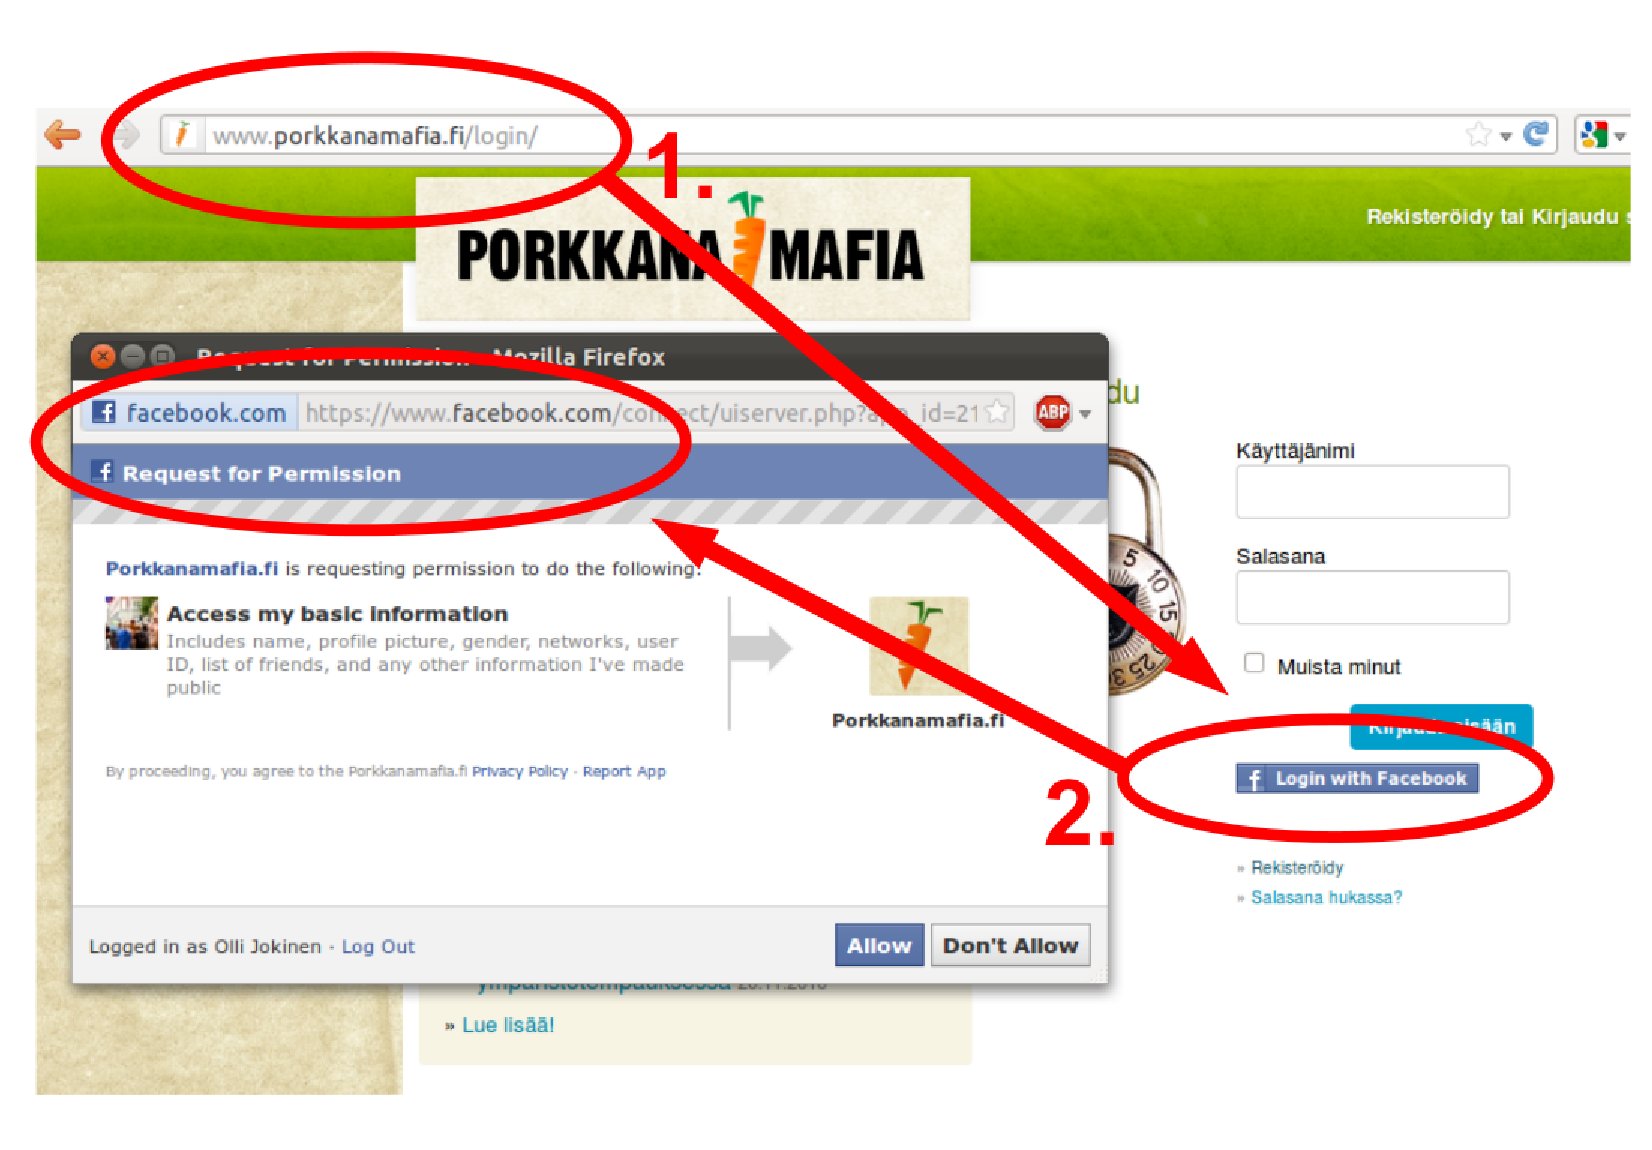
\includegraphics[width=\textwidth]{teknologiat/facebook.eps}
\caption{Käyttäjän kirjautuminen Facebook-tunnuksilla Porkkanamafian web-palveluun}%
\label{facebook_login}
\end{figure}

Samaa periaatetta voidaan käyttää myös organisaatioiden sisäisessä tunnistautumispalvelussa. Organisaation sisäiseen palvelusuuntautuneeseen arkkitehtuuriin toteutetaan erillinen web-palvelu, joka on yhteydessä olemassa olevaan käyttäjätietokantaan (esim. LDAP), ja tarjoaa Facebookia vastaavan tunnistautumisen.

Keskitetty tunnistautumispalvelun periaate on kuvattu kuvassa \ref{composition}, jossa on neljä palveluun kuuluvaa komponenttia. Ensimmäiseksi käyttäjä menee WWW-selaimen avulla web-palveluun, joka pyytää tunnistautumista erillisessä tunnistautumispalvelussa. Käyttäjän selain ohjataan tunnistautumispalvelun sivulle, joka on yhteydessä organisaation käyttäjähallintaan. Jos käyttäjähallinnasta löytyy käyttäjän syöttämät tunnistetiedot, palautetaan käyttäjälle valtuutusavain, jonka käyttäjä lähettää takaisin web-palvelulle. Tämän jälkeen web-palvelu varmistaa tunnistautumispalvelulta valtuutusavaimen oikeellisuuden ja tunnistautumispalvelu palauttaa käyttäjän tiedot web-palvelulle.

\begin{figure}[ht]
\centering
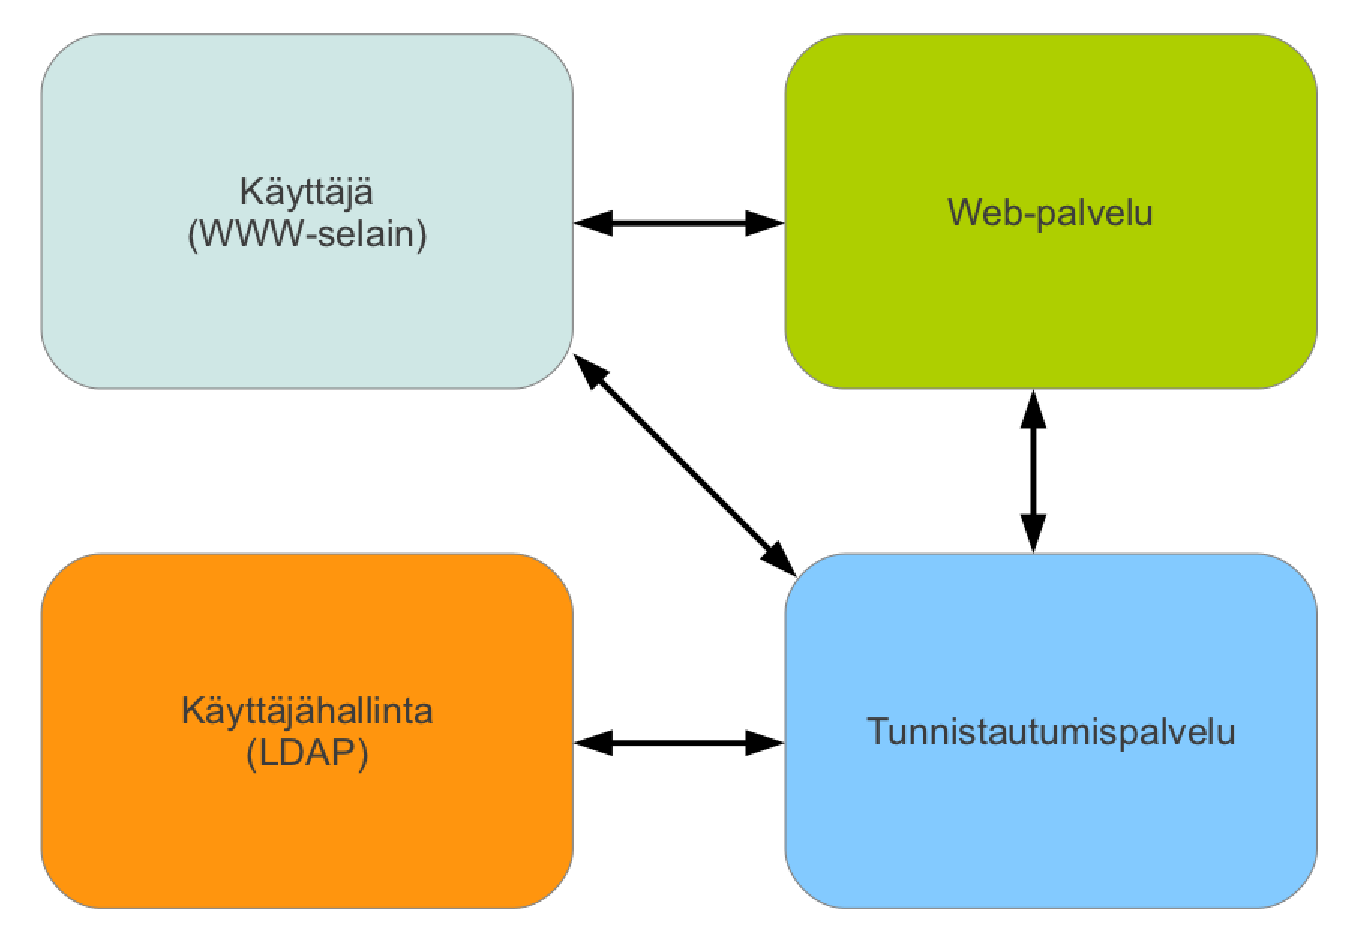
\includegraphics[width=\textwidth]{teknologiat/composition.eps}
\caption{Keskitetyn tunnistautumisen periaatteet}%
\label{composition}
\end{figure}

\subsection{Keskitetyn tunnistautumisen rajapintaprotokollat}
Miten käyttäjädataa onko käsitelty ja käsitellään. Kehitys paikallisesti käytetyistä tiedostopohjaisista systeemeistä kohti tietokantoja ja asiaan räätälöihin palveluihin (LDAP). LDAP oleelisin, mutta tutkimuksen kannalta abstraktointi on tärkeä juttu.

Johdanto puoli sivua, alaluvut 0.5-1 sivu.
\subsubsection{Kerberos}
Lähteet:
Enhancing Distributed Web Security Based on Kerberos Authentication Service (\cite{enchancing_distributed_web_security})
Secure Secret-Key Management of Kerberos Service (\cite{secure_secret_key})

Kerberos-protokolla on alunperin MIT:ssa kehitetty tunnistautumisprotokolla, jonka nykyisin käytössä oleva versio 5 julkaistiin alunperin syyskuussa 1993 ja päivitettynä heinäkuussa 2005 [RFC4120]. Se on yleisesti käytössä erilaisissa UNIX-pohjaisissa käyttöjärjestelmissä ja myös Microsoft on käyttänyt sitä oletus-tunnistautumismekanismina Windows 2000:sta lähtien [RFC3244].

Protokollan osapuolia ovat käyttäjä, luotettava kolmas osapuoli ja palvelu, joka vaatii tunnistautumisen. Luotettava kolmas osapuoli on tyypillisesti avaintenjakopalvelin (KDC, Key Distribution Center), joka tunnistaa käyttäjän ja myöntää lipun tunnistautuneelle käyttäjälle. Myönnettyyn lippuun on merkattu palvelu, johon sitä voidaan käyttää ja aikaleima, jonka ajan se on voimassa. Käyttäjä antaa lipun tunnistautumista vaativalle palvelimelle, joka tarkistaa omalla avaimellaan käyttäjän tunnisteen ja aikaleiman, joiden perusteella se myöntää pääsyn palveluun.

Keskitetty tunnistautuminen hajautettuihin järjestelmiin voidaan toteuttaa Kerberos-protokollalla \cite{enchancing_distributed_web_security}. Kerberos on luonteeltaan sopiva hajautettuihin järjestelmiin, koska avaintenjakopalvelin voi jakaa lippuja kaikkiin järjestelmiin, joiden kanssa se on vaihtanut salausavaimet. Tunnistautumispalvelin on tilaton, jolloin sen suorituskykyä voidaan parantaa tarvittaessa skaalaamalla, joten tunnistautumispalvelin voi palvella suurta määrää käyttäjiä \cite{enchancing_distributed_web_security}.

Tunnistautumisessa käytetyt yksityiset avaimet tallennetaan tietokantaan, jolloin on riskinä, että kolmas osapuoli saattaa päästä käsiksi näihin avaimiin ja pystyä allekirjoittamaan lippuja. Jakamalla salaiset avaimet osiin ja hajauttaa se avaintenjakopalvelimeen, tunnistautumista vaativalle palvelimelle ja näiden välillä käytetylle reitittimelle \cite{secure_secret_key}, voidaan parantaa protokollan luotettavuutta. Tämä tekee siitä mahdollisen vaihtoehdon käytetyksi menetelmäksi keskitettyyn tunnistautumiseen hajautetuissa järjestelmistä.

\subsubsection{SAML}
Security Assertion Markup Language (SAML) on OASIS-komitean kehittämä XML-pohjainen avoin standardi tunnistautumiseen ja pääsynhallintaan \cite{saml_spec}. Standardin versio 1.0 julkaistiin marraskuussa 2002, versio 2.0 maaliskuussa 2005 ja viimeksi päivitetty versio lokakuussa 2009.

SAML määrittelee XML-pohjaiset työkalut tunnistautumisen ja pääsynhallinnan toteuttamiseen. Varsinainen toteutus, esimerkiksi mitä tietoja siirretään ja millä tavalla, jätetään SAML:ssä toteuttajan päätettäväksi \cite{dynamic_saml}. Varsinaiset SAML-viestit voivat kulkea esimerkiksi synkronisesti SOAP- ja HTTP-protokollalla. SAML soveltuu avoimena ja XML-pohjaisena protokollana käytettäväksi Web Services -standardilla toteutetuissa web-sovelluksissa.

Noin sivu lisää, jotta selviää mikä SAML loppujen lopuksi on.
\subsubsection{OAuth}
OAuthin kehitystyö alkoi marraskuussa 2006, kun Twitter-pal\-ve\-luun toteutettiin \mbox{OpenID-tukea}. Pian huomattiin, ettei OpenID sovellu käytettäväksi palvelun API-ra\-ja\-pin\-to\-jen kanssa, vaan tarvittiin erillinen pääsynvalvontaprotokolla \cite{oauth_primer}. Siihen asti Twitter-integraatio oli toteutettu pyytämällä käyttäjää antamaan Twitter-tun\-nuk\-sen\-sa ja -salasanansa, joiden avulla palvelu integroitui käyttäjän Twitter-tiliin. Twitterin kehittämä xAuth ja siitä kehittynyt OAuth-protokolla mahdollistavat resurssien käytön ilman käyttäjätunnuksen ja salasanan luovuttamista kolmannelle osapuolelle \cite{oauth2_0}.

OAuthin ensimmäinen versio (1.0) julkaistiin lokakuussa 2007 ja päivitetty versio (1.0a) kesäkuussa 2009 \cite{oauth2_0}. OAuthin versio 2.0 on myös kehitteillä ja se on tarkoitus julkaista marraskuussa 2012 \cite{oauth2_0}. OAuth on määritelty RFC-dokumentissa numero 5849. OAuthin 2.0-version kehitys on ollut vaikeuksissa lähinnä sen jatkuvasti kasvaneiden ominaisuusvaatimusten takia. OAuth 2.0 on kuitenkin käytössä useissa palveluissa, kuten Facebookissa ja GitHubissa, koska OAuth 1.0a:n ominaisuudet eivät ole riittäneet niille. 2.0 helpottaa mm. API-kutsujen tekemistä, koska valtuutusavainten allekirjoitusta on yksinkertaistettu \cite{oauth2_0}.

OAuth on avoin pääsynvalvontaprotokolla hajautetuille web-sovelluksille. Se mahdollistaa käyttäjien resurssien jakamisen palveluiden välillä ilman käyttäjätunnuksen tai salasanan luovuttamista kolmansille osapuolille. Se perustuu erilaisten valtuutusavainten välittämiseen palveluiden kesken \cite{oauth2_0}. Valtuutusavain on allekirjoitettu identiteetintarjoajalla, johon sekä käyttäjä että palvelun toteuttaja luottaa. Muun muassa Facebook tarjoaa avoimen OAuth-rajapinnan, jota web-sovellusten toteuttajat voivat käyttää pääsynvalvonnassaan.

Kuvassa \ref{oauth} on esitetty, kuinka OAuthia käytetään käyttäjän tunnistamiseen. Tunnistautumispalvelin ja käyttäjähallinta voidaan toteuttaa erillisinä palveluina. Tällöin tunnistautumispalvelun antaa pääsyvaltuuden web-sovellukselle, jonka avulla tiedot haetaan käyttäjähallinnasta (kohdat 10 ja 11). Selkeyden vuoksi tunnistautumispalvelun oletetaan toimivan myös käyttäjätietojen jakelijana.

\begin{figure}[!b]
\centering
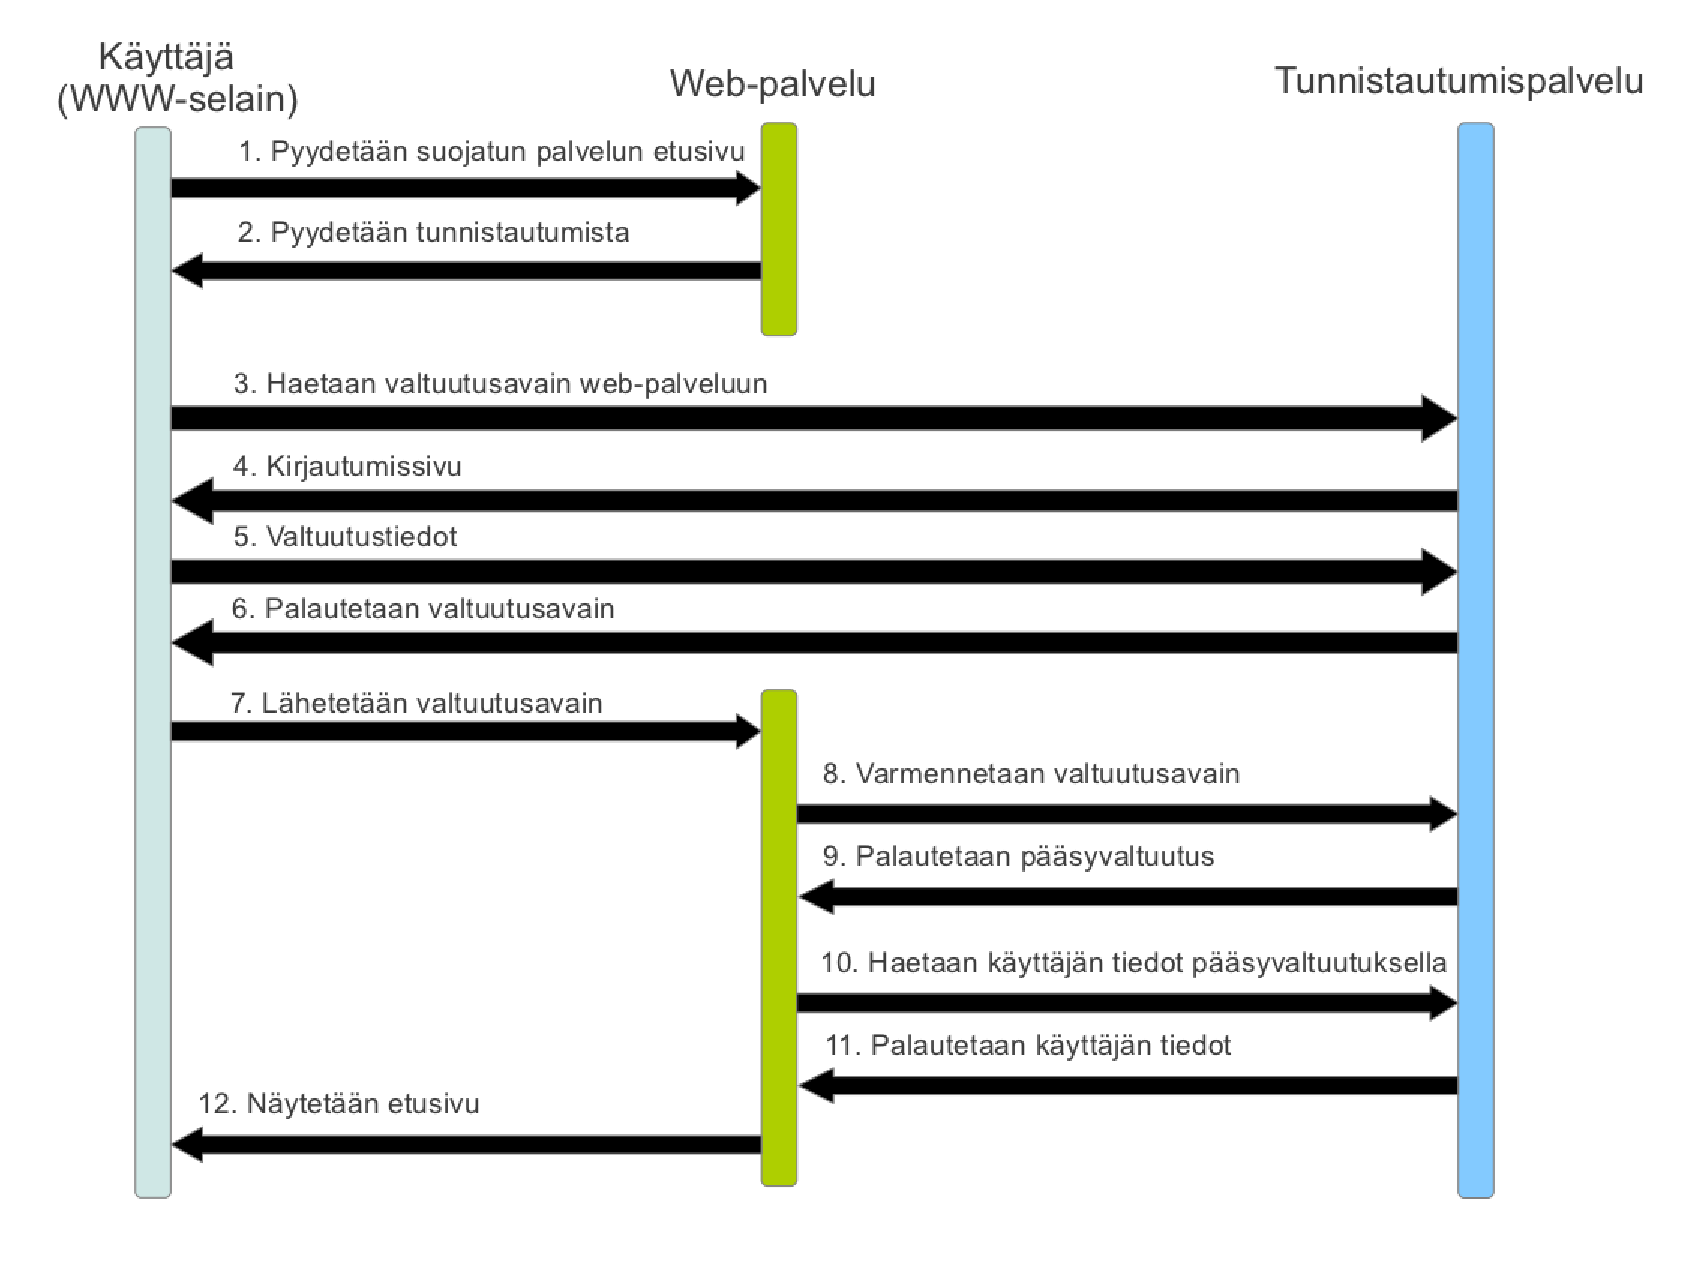
\includegraphics[width=\textwidth]{teknologiat/protokollat/oauth.eps}
\caption{OAuthin toiminta sekvenssikaaviona.}%
\label{oauth}
\end{figure}

OAuthissa valtuutusavaimelle voidaan asettaa erilaisia rajoituksia esimerkiksi sen suhteen, mitä tietoja käyttäjästä annetaan web-sovellukselle tai mihin resursseihin kyseisellä avaimella pääsee käsiksi. Kuvassa \ref{facebook_login} kirjautumisen yhteydessä Porkkanamafialle annetaan oikeus nähdä käyttäjän nimi, profiilikuva, sukupuoli jne. OAuth ei siis ole varsinaisesti tunnistautumisprotokolla, mutta valtuutusavaimen perusteella käyttäjä voidaan yksilöidä: kun käyttäjä kirjautuu myöhemmin uudestaan Porkkanamafiaan, hän hakee valtuutusavaimen Facebookilta, jota käyttämällä Porkkanamafia hakee Facebookista käyttäjän tiedot. Käyttäjän tiedoissa mukana olevalla Facebookin yksilöivällä tunnistenumerolla käyttäjä voidaan todeta samaksi kuin edellisellä kirjautumiskerralla.
\subsection{Yhteenveto}
Keskitetyn tunnistautumispalvelun käyttö on perusteltua, jos ympäristössä on useita käyttäjän tunnistamista vaativia web-sovelluksia. Tunnistautumispalvelun käytöllä ehkäistään käyttäjätietojen kopiointiin liittyviä synkronointiongelmia, kun käyttäjädata on keskitetty yhteen paikkaan. Erityisesti arkaluontoinen data, kuten salasanatiivisteet, kannattaa keskittää, jolloin ne eivät päädy vääriin käsiin yksittäisiin web-sovelluksiin kohdistuneiden tietomurtojen yhteydessä.

Tunnistautumispalvelu mahdollistaa myös muiden kuin järjestelmän ylläpitäjien tuottamien sovellusten käytön organisaation sisäisillä käyttäjätunnuksilla. Käyttämällä luotettavaksi todettuja rajapintoja, voi ylläpito antaa kolmannen osapuolen toteuttamalle web-sovellukselle oikeuden käyttää tunnistautumispalvelua käyttäjän tunnistamiseen. Tällöin käyttäjä ohjataan tunnistautumispalveluun tunnistamisen ajaksi ja web-sovellus saa vain pääsyvaltuuden, jolla sovellus voi hakea käyttäjän tiedot. Käyttäjän tunnistetiedot eivät tule missään vaiheessa tunnistamista tarvitsevan web-sovelluksen tietoon. Näin ollen esimerkiksi Facebook-tunnuksilla voi kirjautua useaan web-sovellukseen, vaikka Facebookilla ei ole tarkkaa tietoa sovelluksien sisäisestä toimintalogiikasta.

Tutkielmassa esitellyn Kapsi ry:n hallintatyökalujen tapauksessa palvelu tullaan toteuttamaan Django-sovelluskehyksellä, mutta myös valmiita toteutuksia on olemassa eri intranet-ympäristöihin. Teknologivalinta tulee tehdä sovellusympäristön mukaan, eikä yksi ratkaisu sovi kaikkiin ympäristöihin. Web-sovelluksen ja tunnistautumispalvelun välinen rajapinta pitää huolen palveluiden yhteensopivuudesta. Rajapinnoiksi on valittavissa useita eri protokollia, kuten Web Services -standardin SAML tai avoimen lähdekoodin yhteisössä syntyneet OpenID ja OAuth. Protokollien käyttö rinnakkain on myös mahdollista, jolloin tunnistautuminen voidaan tehdä esimerkiksi SAML- tai OAuth-protokollalla riippuen web-sovelluksesta.

Tunnistautumiseen liittyvien tehtävien erottaminen yksittäisiltä web-sovelluksilta erillisen palvelun tehtäväksi on palvelusuuntauneiden arkkitehtuurien periaatteiden mukaista. Tällaisten arkkitehtuurien mukaan toteutetuissa sovellusympäristöissä jokaisella web-sovelluksella on oma tarkasti määritelty tehtävä. Kun arkkitehtuurissa on oma palvelu tunnistautumiselle, on pienten yksittäisten komponenttien toteutus helpompaa, koska jokaisen komponentin kohdalla ei tarvitse huolehtia tunnistautumisen toteutuksesta.

Web-sovelluksen ja tunnistamisen erottaminen toisistaan mahdollistaa myös tunnistautumisen tehostamisen ilman muutoksia web-sovellusten toimintaan. Järjestelmässä voidaan ottaa salasanan lisäksi käyttöön toiseen tekijään perustuva tunnistaminen, jolloin esimerkiksi käyttäjän täytyy salasanan lisäksi syöttää matkapuhelimeen lähetetty tunnistekoodi. Web-sovelluksen ja tunnistautumispalvelun välinen rajapinta ei tässä tapauksessa muutu, joten tunnistamisen parantaminen ei edellytä web-sovelluksien muuttamista.

Keskitetyn pääsynvalvonnan toteuttaminen tutkielmassa kuvatuilla periaatteilla on mahdollista. Tällöin tiedot käyttäjien pääsyoikeuksista ympäristön sisällä ovat yhdessä paikassa, joka helpottaa niiden hallinnointia. Esimerkiksi henkilön siirtyessä tehtävästä toiseen, voidaan hänen pääsyvaltuudet muuttaa samasta paikasta. Pääsynvalvontaan voidaan käyttää esimerkiksi tutkielmassa esiteltyjä SAML- tai OAuth-protokollia.

Käyttäjän tunnistamista vaativissa web-sovelluksissa käyttäjän tunnistaminen kannattaa toteuttaa erillisenä komponenttina. Käytettyjen teknologioiden suhteen valinta täytyy tehdä web-sovellusympäristön mukaan, koska kaikkiin ympäristöihin sopivaa ratkaisua ei ole. Tässä tutkielmassa esitellyt periaatteet ovat kuitenkin sovellettavissa eri teknologioita käytettäessä.

\section{Toteutus}
Toteutuksen kuvaus. Arkkitehtuuri yms, koodi liitteenä jos tarvii?

Käytännössä kyseessä on palveluna toimiva tunnistautumisjärjestemä, jolla on joku tietokanta ja rajapinta, jonka kautta tunnistautumispyyntöjä tehdään. Todennäköisesti käyttäjätietokanta on relaatiokanta ja rajapinta Oauth.

Tässä luvussa kuvataan ko. toteutus tarpeellisella tarkkuudella. Järjestelmän arkkitehtuuria, viestinkulkua yms kuvataan UML-tekniikalla.

Tutkielman tarkoitus on toteuttaa prototyyppi sovelluksesta, jonka avulla erillisten web-sovellusten käyttäjähallinta keskitetään yhteen komponenttiin. Sovellus hoitaa käyttäjän tunnistautumisen ja käyttäjätietojen hallinnan, joka synkronoidaan asiakasyrityksen käyttäjätietokannan kanssa. 

Pituus n. 10sivua.

\section{Toteutuksen evaluaatio}
Tutkielman (erityisesti luvun 5) kriittinen arviointi, osattiinko esitellyllä arkkitehtuurilla vastata johdannossa esitettyihin kysymyksiin.

Vielä hieman auki, mutta pituus noin 5 sivua.

Tutkielmassa ei keskitytä kaikille avoimiin tunnistautumispalveluihin (kuten Facebook tai Google), vaan organisaatioihin, joilla on oma käyttäjähallinta. Esimerkki tällaisesta organisaatiosta on Helsingin yliopisto, jolla on oma Active Directory -käyttäjähallinta \cite{tietotekniikkaa}. Myös monet yritykset ylläpitävät omaa käyttäjähallintaa esimerkiksi LDAP-järjestelmässä tai keskitetyssä tietokannassa. Esimerkkinä hyötyjä ja haittoja punnittaessa käytetään Helsingin yliopistoa, mutta myös muunlaiset organisaatiot huomioidaan, mikäli se on perusteltua. TODO: tämä kappale uusiksi, kun 5-7 hahmottuu

\subsection{Esimerkkiarkkitehtuurin laajennettavuus}
Kuinka voisi laajentaa? Kertakirjautuminen ja autorisointi hyviä suuntia. SSO aika peruskamaa OAuthin kanssa, autorisoinnista sen sijaan voi saada ihan mielenkiintoista pohdintaa aikaan.

LDAP:n hyödyntäminen autorisoinnissa, voisiko esimerkiksi käyttäjäryhmät olla tallennettu jotenkin kätevästi LDAP:in ja niiden perusteella voidaan autorisoida pääsy resurssiin.

Sinällään pääsynhallinta tiettyihin palveluihin on jonkin tason autorisointia ja kuuluu ehdottomasti gradun aihepiiriin (toteutus tunnistaa x:n palvelun käyttäjiä samaa käyttäjädataa vasten, kaikille käyttäjille ei saa antaa oikeutta kaikkiin palveluihin).

Miten käyttäjädataa onko käsitelty ja käsitellään. Kehitys paikallisesti käytetyistä tiedostopohjaisista systeemeistä kohti tietokantoja ja asiaan räätälöihin palveluihin (LDAP). LDAP oleelisin, mutta tutkimuksen kannalta abstraktointi on tärkeä juttu.

Johdanto puoli sivua, alaluvut 0.5-1 sivu.
\subsection{Kertakirjautuminen}
Kertakirjautumisella (SSO) tarkoitetaan arkkitehtuuria, jossa yhdellä kirjautumisella tunnistaudutaan useaan eri palveluun \cite{sso}. Käytetyissä kertakirjautumistekniikoissa käytetään identiteetintarjoajaa (identity provider), joka varmentaa kirjautumisen ja luo valtuutuksen web-sovellukseen. Käytetyt tekniikat jaetaan kahteen osaan: näennäiseen- (pseudo SSO) ja tosikertakirjautumiseen (true SSO) \cite{sso}. Näennäisessä kertakirjautumisessa identiteetintarjoaja luo palveluun sopivan valtuutuksen, jolloin web-sovellus ei tiedä kertakirjautumisesta mitään. Tosikertakirjautumisessa taas käytetään yleisiä järjestelmänlaajuisia valtuutuksia, jolloin web-sovellusten täytyy olla tietoisia kertakirjautumisesta.

Kapsin nykyisessä arkkitehtuurissa käyttäjä voi kirjautua samalla tunnuksella eri palveluihin, mutta kyseessä ei ole kertakirjautuminen, koska kirjautumisen täytyy tehdä erikseen jokaiseen palveluun. Kertakirjautuminen on mahdollista tehdä myös nykyisessä arkkitehtuurissa, esimerkiksi tallentamalla tunnistetiedot selaimen evästeeseen (cookie). Toinen web-sovellus voi taas lukea tunnistetiedot evästeestä ja tunnistaa käyttäjän tätä kautta. Koska eri web-sovellukset toimivat samassa domain-osoitteessa, ne voivat lukea toistensa kirjoittamia evästeitä \cite{rfc6265}. Tällainen ratkaisu on kuitenkin ongelmallinen, koska tunnistetiedot tallennetaan käyttäjän koneelle ja ne on luettavissa evästeestä. Jos taas tunnistetietojen kirjoittamiseen ja lukemiseen käytetään salausta, joudutaan salausavain jakamaan web-sovellusten kesken. Tämä lisää ylläpidon tarvetta.

Keskitettyä tunnistautumispalvelua käytettäessä kertakirjautuminen voidaan toteuttaa OAuth-protokollalla \cite{distributed_web_security}. Kontrollin kulku on samanlainen kuin kuvassa \ref{auth_kapsi_fi_flow}, mutta käyttäjän ei tarvitse syöttää tunnusta ja salasanaa, koska hänellä on jo voimassaoleva istunto tunnistautumispalveluun. Toisin sanoen käyttäjäagentti (selain) saa pääsyvaltuuden tunnistautumispalvelusta ilman uutta kirjautumista, jolloin kyseessä on näennäinen kertakirjautuminen. Kuitenkin ensimmäistä kertaa kirjautuessa web-sovellukseen käyttäjän täytyy hyväksyä tietojen haku tunnistautumispalvelusta. Kun tietojen luovutus on hyväksytty, voidaan jatkossa kirjautuminen tehdä ilman käyttäjän syötettä.
\subsection{Autorisointi}
Esitetyssä arkkitehtuurissa OAuth-protokollaa käytetään tunnistautumisen toteuttamiseen, mutta sen käyttöä voidaan laajentaa myös muuhun pääsynvalvontaan \cite{distributed_web_security}. Käyttö on varsin perusteltua, sillä OAuth on nimenomaan pääsynvalvontaprotokolla ja tunnistamisen toteuttaminen sitä käyttäen on erikoiskäyttötapaus. OAuthia käyttäen tunnistautumispalvelu voidaan laajentaa suojaamaan Kapsin järjestelmissä käytettäviä resursseja.

Jäsenen tiedot voivat olla yksi resurssi, joiden käyttöä valvotaan auth.kapsi.fi-pal\-ve\-lun kautta. Tällöin Sikteeri saa käyttäjätietokannasta tiedot vain, jos käyttäjällä olisi esittää pääsyvaltuutus, joka oikeuttaa tietojen hakemiseen. Näin Sikteeri ei olisi suoraan yhteydessä käyttäjätietokantaan, vaan arkkitehtuuriin lisätään palvelu, joka mahdollistaa käyttäjän hakemisen, lisäämisen, muokkaamisen tai poistamisen. Tämä palvelu on yhteydessä LDAP-käyttäjätietokantaan ja se antaa lukea tietoja vain jos käyttäjällä on esittää oikea pääsyvaltuutus. Pääsyvaltuuksia hallinnoi tunnistautumispalvelu.

Arkkitehtuurin laajentaminen koskemaan myös pääsynvalvontaa veisi sitä entistä enemmän kohti palveluperusteista arkkitehtuuria, jossa jokaisella komponentilla on yksi tehtävä, jonka ne suorittavat hyvin \cite{soa}. Sikteeri olisi siinä tapauksessa käyttöliittymä komponentille, joka hallinnoi käyttäjiä. Päätös käyttäjän oikeudesta hallinnoida käyttäjiä ei ole Sikteerin vastuulla vaan vastuu on keskitetty omaan palveluun.

Pääsynvalvonnan keskittäminen on perusteltua, koska silloin käyttäjien oikeuksiin liittyviä toimenpiteitä on helpompi tehdä. Esimerkiksi toimihenkilön siirtyessä rivijäseneksi, ei hänen käyttöoikeuksia tarvitse poistaa jokaisesta Kapsin palvelusta, vaan pelkästään keskitetystä pääsynvalvonnasta. Toistaiseksi ongelma ei ole kovin suuri, koska palveluita on vain kaksi, mutta varsinkin kun arkkitehtuuria viedään kohti kuvassa \ref{kapsi_uusi} esitettyä palveluperustaista arkkitehtuuria, tarve korostuu.

\subsection{Toteutuksen rajoitukset}
Kun Kapsin tietojärjestelmissä siirrytään keskitetyn tunnistautumispalvelun käyttöön, joudutaan tunnistautumista vaativat web-sovellukset muuttaa käyttämään uutta tunnistautumisjärjestelmää. Ohjelman toiminnan kannalta tällä ei saavuteta varsinaisesti mitään hyötyä, joten kyseessä on epätoivottu heijastusvaikutus (ripple effect). Heijastusvaikutuksella tarkoitetaan muutoksia, joita joudutaan tekemään ohjelmaan, joita alkuperäiset muutokset eivät suoraan koske \cite{arkkitehtuurit}. Toisaalta ratkaisulla vähennetään heijastusvaikutuksia tulevaisuudessa, kun web-sovelluksen ja tunnistautumisen välinen vahva riippuvuussuhde puretaan \cite{arkkitehtuurit}. Tällöin esimerkiksi kaksivaiheisen kirjautumisen toteuttaminen järjestelmään ei vaadi muutoksia kirjautumista käyttäviin web-sovelluksiin.

Esimerkkiarkkitehtuuri kasvattaa myös jonkun verran järjestelmän kompleksisuutta, kun käytössä olevien komponenttien määrä kasvaa. Myös tunnistautumispalvelun toteutuksessa käytetty tekniikka saattaa poiketa sitä käyttävien web-sovellusten tekniikasta, joka kasvattaa kompleksisuutta entisestään \cite{arkkitehtuurit}. Tällä hetkellä ongelmaa ei ole, sillä Kapsin järjestelmissä käytetään yleisesti Django-ohjelmistokehystä, jolla myös tunnistautumispalvelu toteutetaan. Jos jatkossa siirrytään toisiin web-ohjelmointikehyksiin, voi tunnistautumispalvelusta tulla perinnejärjestelmä, jonka muuttamiseen yhdistyksessä ei ole ammattitaitoa. Tämä on kuitenkin erittäin epätodennäköinen skenaario, koska web-palvelun ja tunnistautumispalvelun välinen rajapinta varmistaa, että tunnistautumispalvelu voidaan kirjoittaa helposti uusiksi, ilman heijastusvaikutuksia web-sovelluksiin, ennen kuin Django on muuttunut perinnetiedoksi.

\subsection{Soveltamisalueet}
Miten käyttäjädataa onko käsitelty ja käsitellään. Kehitys paikallisesti käytetyistä tiedostopohjaisista systeemeistä kohti tietokantoja ja asiaan räätälöihin palveluihin (LDAP). LDAP oleelisin, mutta tutkimuksen kannalta abstraktointi on tärkeä juttu.

Johdanto puoli sivua, alaluvut 0.5-1 sivu.

\subsubsection{Keskitetty tunnistautuminen Helsingin yliopiston tietojenkäsittelytieteen laitoksella}
Case-esimerkistä saadun kokemuksen perusteella keskitettyä tunnistautumisratkaisua voitaisiin hyödyntää myös Helsingin yliopiston tietojenkäsittelytieteen laitoksella. Tällä hetkellä laitoksen opiskelijoiden käytössä on erilaisia web-palveluita, kuten kurssi-ilmoittautuminen ja sähköposti. Lisäksi henkilökunnalla on palveluita mm. kurssisuoritusten ylläpitoa varten. Nämä palvelut voisivat olla yhteydessä keskitettyyn tunnistautumispalveluun, jolloin niiden ei tarvitsisi päästä suoraan käyttäjähallintaan.

Edellisen lisäksi keskitetty tunnistautumispalvelu mahdollistaisi muiden kuin laitoksen IT-osaston tuottamien web-palveluiden käytön laitoksen käyttäjätunnuksilla. Ohjelmistotuotantoprojekti-kurssin opiskelijat voisivat tuottaa web-palveluita laitoksen opiskelijoiden ja henkilökunnan käyttöön. Esimerkiksi keväällä 2010 toteutettu opiskelijoiden ainejärjestö TKO-älyn rekrytointipalvelu olisi voinut käyttää hyväkseen keskitettyä tunnistautumispalvelua, jolloin käytön rajaaminen vain laitoksen opiskelijoiden käyttöön olisi ollut mahdollista. Laitoksen LDAP-käyt\-tä\-jä\-hal\-lin\-nan käyttö tunnistautumiseen ei tullut kysymykseen, koska se olisi ollut tietoturvariski. Keskitettyä tunnistautumispalvelua käytettäessä riskiä ei ole, sillä web-palvelun tietokantaan tallennetaan vain yksilöivä käyttäjätunnus ja tunnistautuminen tehdään tunnistautumispalvelussa.

Myös keskitetystä pääsynvalvonnasta olisi hyötyä tietojenkäsittelytieteen laitoksen tapauksessa. Laitoksella on erilaisia ryhmiä, esimerkiksi kantahenkilökunta, tutkijat, sivutoimiset tuntiopettajat, vierailevat luennoitsijat, joilla on käytössään erilaisia palveluita. Tutkijat voivat käyttää Ukko-laskentaklusteria, sivutoimiset tuntiopettajat ja muu opetushenkilökunta kirjata arvosanoja kurssikirjanpitojärjestelmään jne. Näiden kaikkien palveluiden pääsynvalvonta olisi perusteltua toteuttaa keskitetysti, jolloin henkilön roolin muuttuessa hänen käyttöoikeuksien muuttaminen olisi helppoa. Keskitetyn tunnistautumispalvelun käyttöönoton jälkeen myös pääsynvalvonta voitaisiin keskittää luvussa 6.3.1 mainitulla tavalla.

\subsubsection{Keskitetty tunnistautuminen yrityksen intranetissä}
TODO: tähän on tosi vaikea löytää mitään viitteitä

Yritysten intranet-järjestelmät muistuttavat usein Kapsin arkkitehtuuria: järjestelmässä on erilaisia web-palveluita, joihin kirjaudutaan sisäisellä käyttäjätunnuksella. Keskitetyn tunnistautumispalvelun tuominen tällaiseen järjestelmään on perusteltua samoista syistä kuin Kapsin tapauksessa.

Usein yrityksissä ei toteuteta web-palveluita itse, vaan käytetään valmiita ratkaisuja. Tällöin keskitetyn tunnistautumispalvelun teknologiavalinnat täytyy tehdä ympäristön mukaan. Esimerkiksi jos intranet-palvelu on rakennettu Microsoftin SharePoint-teknologialla, on tunnistautumispalvelu toteutettavissa Microsoftin teknologialla \cite{sharepoint}. Myös muilla teknologioilla toteutettuihin intranet-järjestelmiin on tarjolla kaupallisia keskitettyjä tunnistautumisratkaisuja, esimerkiksi suomalaisen Ubisecuren CustomerID \cite{ubisecure}. [TODO: maksettu mainos? joku open source tilalle?]

Jos taas yrityksessä tuotetaan intranetin palveluita itse, voi oman tunnistautumispalvelun toteuttaminen Kapsin tapaan olla perusteltua. Usein omien palveluiden lisäksi järjestelmässä käytetään muiden tuottamia palveluita esimerkiksi sähköpostia varten. Tällöin täytyy selvittää teknologioiden yhteensopivuus valmiiden palveluiden kanssa, jolloin esimerkiksi SAML voi osoittautua OAuthia paremmaksi ratkaisuksi tunnistautumisen rajapintaprotokollaksi.

\subsubsection{Tunnistautuminen web-sovelluksissa ilman omaa käyttäjähallintaa}
Keskitetyn tunnistamisen periaatteita voidaan soveltaa myös ilman omaa käyttäjähallintaa. Tällöin web-sovellukseen kirjautuminen vaatii, että käyttäjällä on tunnus tunnistautumisen tarjoavan kolmannen osapuolen palveluun, esimerkiksi Facebookiin tai Googleen. Näillä ja monilla muilla palveluntarjoajilla on käytössään OAuth-pohjainen tunnistautumisrajapinta \cite{inside_the_identity_management_game}.

Ulkoistetun käyttäjähallinnan hyvänä puolena voidaan pitää sen vaivattomuutta. Tunnistamista tarjoavilla palveluilla on tapa varmistaa käyttäjän tiedot, joten web-sovelluksen ylläpitäjän ei tarvitse varmistaa niiden oikeellisuutta. Käyttäjät päivittävät tietonsa mielummin Facebookiin tms. kuin yksittäisiin web-palveluihin, joten tieto pysyy tuoreempana \cite{inside_the_identity_management_game}. Lisäksi web-sovelluksen ylläpitäjän pelko joutua salasanamurtojen kohteeksi vähenee, koska palveluun ei tallenneta salasanoja (tai edes niiden tiivisteitä).

Haittapuolena ulkoisesta tunnistamispalvelusta on, että käyttäjällä täytyy olla tunnus kolmannen osapuolen palveluun, jotta hän voi kirjautua web-sovellukseen. Vaikka Facebookilla ja Googlella on merkittävä määrä rekisteröityneitä käyttäjiä, jää niiden ulkopuolelle useita ihmisiä. Esimerkiksi Helsingin yliopisto ei voi edellyttää, että sen palveluiden käyttäjillä on tunnus Facebookiin tai Googleen, vaan palveluiden täytyy olla kaikkien opiskelijoiden käytössä. Tällöin oman käyttäjähallinnan rakentaminen ja ylläpito on tarpeen.

Ulkoinen käyttäjähallinta on kuitenkin hyvä ratkaisu monissa tapauksissa. Esimerkiksi monissa verkkolehdissä ja -blogeissa kommentointi on mahdollista vain Fa\-ce\-book-käyt\-tä\-jil\-le, jolloin keskusteluun voivat osallistua vain Facebookin varmentamat käyttäjät. Tällöin anonyymi kommentointi jää pois ja kommentointi tapahtuu vain ihmisten oikeilla nimillä. Ulkoisen käyttäjähallinnan käyttö lisää myös käyttäjien aktiivisuutta palvelussa: yksittäisen web-sovelluksen salasana unohtuu helposti, mutta yleisesti käytetyn sovelluksen salasana muistetaan paremmin \cite{password_habits}.
\section{Toteutuksen laajennettavuus}
Kuinka voisi laajentaa? Kertakirjautuminen ja autorisointi hyviä suuntia. SSO aika peruskamaa OAuthin kanssa, autorisoinnista sen sijaan voi saada ihan mielenkiintoista pohdintaa aikaan.

LDAP:n hyödyntäminen autorisoinnissa, voisiko esimerkiksi käyttäjäryhmät olla tallennettu jotenkin kätevästi LDAP:in ja niiden perusteella voidaan autorisoida pääsy resurssiin.

Sinällään pääsynhallinta tiettyihin palveluihin on jonkin tason autorisointia ja kuuluu ehdottomasti gradun aihepiiriin (toteutus tunnistaa x:n palvelun käyttäjiä samaa käyttäjädataa vasten, kaikille käyttäjille ei saa antaa oikeutta kaikkiin palveluihin).

Miten käyttäjädataa onko käsitelty ja käsitellään. Kehitys paikallisesti käytetyistä tiedostopohjaisista systeemeistä kohti tietokantoja ja asiaan räätälöihin palveluihin (LDAP). LDAP oleelisin, mutta tutkimuksen kannalta abstraktointi on tärkeä juttu.

Johdanto puoli sivua, alaluvut 0.5-1 sivu.
\subsection{Kertakirjautuminen}
Kertakirjautumisella (SSO) tarkoitetaan arkkitehtuuria, jossa yhdellä kirjautumisella tunnistaudutaan useaan eri palveluun \cite{sso}. Käytetyissä kertakirjautumistekniikoissa käytetään identiteetintarjoajaa (identity provider), joka varmentaa kirjautumisen ja luo valtuutuksen web-sovellukseen. Käytetyt tekniikat jaetaan kahteen osaan: näennäiseen- (pseudo SSO) ja tosikertakirjautumiseen (true SSO) \cite{sso}. Näennäisessä kertakirjautumisessa identiteetintarjoaja luo palveluun sopivan valtuutuksen, jolloin web-sovellus ei tiedä kertakirjautumisesta mitään. Tosikertakirjautumisessa taas käytetään yleisiä järjestelmänlaajuisia valtuutuksia, jolloin web-sovellusten täytyy olla tietoisia kertakirjautumisesta.

Kapsin nykyisessä arkkitehtuurissa käyttäjä voi kirjautua samalla tunnuksella eri palveluihin, mutta kyseessä ei ole kertakirjautuminen, koska kirjautumisen täytyy tehdä erikseen jokaiseen palveluun. Kertakirjautuminen on mahdollista tehdä myös nykyisessä arkkitehtuurissa, esimerkiksi tallentamalla tunnistetiedot selaimen evästeeseen (cookie). Toinen web-sovellus voi taas lukea tunnistetiedot evästeestä ja tunnistaa käyttäjän tätä kautta. Koska eri web-sovellukset toimivat samassa domain-osoitteessa, ne voivat lukea toistensa kirjoittamia evästeitä \cite{rfc6265}. Tällainen ratkaisu on kuitenkin ongelmallinen, koska tunnistetiedot tallennetaan käyttäjän koneelle ja ne on luettavissa evästeestä. Jos taas tunnistetietojen kirjoittamiseen ja lukemiseen käytetään salausta, joudutaan salausavain jakamaan web-sovellusten kesken. Tämä lisää ylläpidon tarvetta.

Keskitettyä tunnistautumispalvelua käytettäessä kertakirjautuminen voidaan toteuttaa OAuth-protokollalla \cite{distributed_web_security}. Kontrollin kulku on samanlainen kuin kuvassa \ref{auth_kapsi_fi_flow}, mutta käyttäjän ei tarvitse syöttää tunnusta ja salasanaa, koska hänellä on jo voimassaoleva istunto tunnistautumispalveluun. Toisin sanoen käyttäjäagentti (selain) saa pääsyvaltuuden tunnistautumispalvelusta ilman uutta kirjautumista, jolloin kyseessä on näennäinen kertakirjautuminen. Kuitenkin ensimmäistä kertaa kirjautuessa web-sovellukseen käyttäjän täytyy hyväksyä tietojen haku tunnistautumispalvelusta. Kun tietojen luovutus on hyväksytty, voidaan jatkossa kirjautuminen tehdä ilman käyttäjän syötettä.
\subsection{Autorisointi}
Esitetyssä arkkitehtuurissa OAuth-protokollaa käytetään tunnistautumisen toteuttamiseen, mutta sen käyttöä voidaan laajentaa myös muuhun pääsynvalvontaan \cite{distributed_web_security}. Käyttö on varsin perusteltua, sillä OAuth on nimenomaan pääsynvalvontaprotokolla ja tunnistamisen toteuttaminen sitä käyttäen on erikoiskäyttötapaus. OAuthia käyttäen tunnistautumispalvelu voidaan laajentaa suojaamaan Kapsin järjestelmissä käytettäviä resursseja.

Jäsenen tiedot voivat olla yksi resurssi, joiden käyttöä valvotaan auth.kapsi.fi-pal\-ve\-lun kautta. Tällöin Sikteeri saa käyttäjätietokannasta tiedot vain, jos käyttäjällä olisi esittää pääsyvaltuutus, joka oikeuttaa tietojen hakemiseen. Näin Sikteeri ei olisi suoraan yhteydessä käyttäjätietokantaan, vaan arkkitehtuuriin lisätään palvelu, joka mahdollistaa käyttäjän hakemisen, lisäämisen, muokkaamisen tai poistamisen. Tämä palvelu on yhteydessä LDAP-käyttäjätietokantaan ja se antaa lukea tietoja vain jos käyttäjällä on esittää oikea pääsyvaltuutus. Pääsyvaltuuksia hallinnoi tunnistautumispalvelu.

Arkkitehtuurin laajentaminen koskemaan myös pääsynvalvontaa veisi sitä entistä enemmän kohti palveluperusteista arkkitehtuuria, jossa jokaisella komponentilla on yksi tehtävä, jonka ne suorittavat hyvin \cite{soa}. Sikteeri olisi siinä tapauksessa käyttöliittymä komponentille, joka hallinnoi käyttäjiä. Päätös käyttäjän oikeudesta hallinnoida käyttäjiä ei ole Sikteerin vastuulla vaan vastuu on keskitetty omaan palveluun.

Pääsynvalvonnan keskittäminen on perusteltua, koska silloin käyttäjien oikeuksiin liittyviä toimenpiteitä on helpompi tehdä. Esimerkiksi toimihenkilön siirtyessä rivijäseneksi, ei hänen käyttöoikeuksia tarvitse poistaa jokaisesta Kapsin palvelusta, vaan pelkästään keskitetystä pääsynvalvonnasta. Toistaiseksi ongelma ei ole kovin suuri, koska palveluita on vain kaksi, mutta varsinkin kun arkkitehtuuria viedään kohti kuvassa \ref{kapsi_uusi} esitettyä palveluperustaista arkkitehtuuria, tarve korostuu.
\section{Yhteenveto}
Keskitetyn tunnistautumispalvelun käyttö on perusteltua, jos ympäristössä on useita käyttäjän tunnistamista vaativia web-sovelluksia. Tunnistautumispalvelun käytöllä ehkäistään käyttäjätietojen kopiointiin liittyviä synkronointiongelmia, kun käyttäjädata on keskitetty yhteen paikkaan. Erityisesti arkaluontoinen data, kuten salasanatiivisteet, kannattaa keskittää, jolloin ne eivät päädy vääriin käsiin yksittäisiin web-sovelluksiin kohdistuneiden tietomurtojen yhteydessä.

Tunnistautumispalvelu mahdollistaa myös muiden kuin järjestelmän ylläpitäjien tuottamien sovellusten käytön organisaation sisäisillä käyttäjätunnuksilla. Käyttämällä luotettavaksi todettuja rajapintoja, voi ylläpito antaa kolmannen osapuolen toteuttamalle web-sovellukselle oikeuden käyttää tunnistautumispalvelua käyttäjän tunnistamiseen. Tällöin käyttäjä ohjataan tunnistautumispalveluun tunnistamisen ajaksi ja web-sovellus saa vain pääsyvaltuuden, jolla sovellus voi hakea käyttäjän tiedot. Käyttäjän tunnistetiedot eivät tule missään vaiheessa tunnistamista tarvitsevan web-sovelluksen tietoon. Näin ollen esimerkiksi Facebook-tunnuksilla voi kirjautua useaan web-sovellukseen, vaikka Facebookilla ei ole tarkkaa tietoa sovelluksien sisäisestä toimintalogiikasta.

Tutkielmassa esitellyn Kapsi ry:n hallintatyökalujen tapauksessa palvelu tullaan toteuttamaan Django-sovelluskehyksellä, mutta myös valmiita toteutuksia on olemassa eri intranet-ympäristöihin. Teknologivalinta tulee tehdä sovellusympäristön mukaan, eikä yksi ratkaisu sovi kaikkiin ympäristöihin. Web-sovelluksen ja tunnistautumispalvelun välinen rajapinta pitää huolen palveluiden yhteensopivuudesta. Rajapinnoiksi on valittavissa useita eri protokollia, kuten Web Services -standardin SAML tai avoimen lähdekoodin yhteisössä syntyneet OpenID ja OAuth. Protokollien käyttö rinnakkain on myös mahdollista, jolloin tunnistautuminen voidaan tehdä esimerkiksi SAML- tai OAuth-protokollalla riippuen web-sovelluksesta.

Tunnistautumiseen liittyvien tehtävien erottaminen yksittäisiltä web-sovelluksilta erillisen palvelun tehtäväksi on palvelusuuntauneiden arkkitehtuurien periaatteiden mukaista. Tällaisten arkkitehtuurien mukaan toteutetuissa sovellusympäristöissä jokaisella web-sovelluksella on oma tarkasti määritelty tehtävä. Kun arkkitehtuurissa on oma palvelu tunnistautumiselle, on pienten yksittäisten komponenttien toteutus helpompaa, koska jokaisen komponentin kohdalla ei tarvitse huolehtia tunnistautumisen toteutuksesta.

Web-sovelluksen ja tunnistamisen erottaminen toisistaan mahdollistaa myös tunnistautumisen tehostamisen ilman muutoksia web-sovellusten toimintaan. Järjestelmässä voidaan ottaa salasanan lisäksi käyttöön toiseen tekijään perustuva tunnistaminen, jolloin esimerkiksi käyttäjän täytyy salasanan lisäksi syöttää matkapuhelimeen lähetetty tunnistekoodi. Web-sovelluksen ja tunnistautumispalvelun välinen rajapinta ei tässä tapauksessa muutu, joten tunnistamisen parantaminen ei edellytä web-sovelluksien muuttamista.

Keskitetyn pääsynvalvonnan toteuttaminen tutkielmassa kuvatuilla periaatteilla on mahdollista. Tällöin tiedot käyttäjien pääsyoikeuksista ympäristön sisällä ovat yhdessä paikassa, joka helpottaa niiden hallinnointia. Esimerkiksi henkilön siirtyessä tehtävästä toiseen, voidaan hänen pääsyvaltuudet muuttaa samasta paikasta. Pääsynvalvontaan voidaan käyttää esimerkiksi tutkielmassa esiteltyjä SAML- tai OAuth-protokollia.

Käyttäjän tunnistamista vaativissa web-sovelluksissa käyttäjän tunnistaminen kannattaa toteuttaa erillisenä komponenttina. Käytettyjen teknologioiden suhteen valinta täytyy tehdä web-sovellusympäristön mukaan, koska kaikkiin ympäristöihin sopivaa ratkaisua ei ole. Tässä tutkielmassa esitellyt periaatteet ovat kuitenkin sovellettavissa eri teknologioita käytettäessä.

\bibliographystyle{tktl}
\bibliography{misc/lahteet}
\lastpage
%\appendices
%\internalappendix{\theappendix}{Eka liite}
%Liitetekstiä.
%\internalappendix{2}{Toka liite}
%Liitetekstiä. Ehkä kuviakin.
%\externalappendix{\theappendix}{Ohjelmalistaus joka ei sisälly \LaTeX-tiedostoon}
\end{document}
